\documentclass[sigconf,anonymous,review]{acmart}

\setcopyright{none}
\settopmatter{printacmref=false}
\renewcommand\footnotetextcopyrightpermission[1]{}
\acmYear{2026}
\acmConference[MiLeTS '26]{The 12th Mining and Learning from Time Series Workshop}{August 2026}{Jeju, Republic of Korea}
\acmBooktitle{The 12th Mining and Learning from Time Series Workshop (MiLeTS '26), held in conjunction with KDD 2026}

\usepackage{booktabs}
\usepackage{multirow}
\usepackage{graphicx}
\usepackage{subcaption}
\usepackage{xcolor}
\usepackage{listings}
\usepackage{tikz}
\usepackage{tabularx}
\usetikzlibrary{shapes.geometric, arrows.meta, positioning, calc, fit, backgrounds}

\lstset{
  basicstyle=\ttfamily\footnotesize,
  breaklines=true,
  columns=fullflexible,
  frame=single,
  framerule=0.4pt,
  rulecolor=\color{black!20}
}


\title[LeNEPA: No-Augmentation Next-Latent Prediction for Time Series]{\texorpdfstring{LeNEPA: No-Augmentation Next-Latent Prediction\\for Time-Series Representation Learning}{LeNEPA: No-Augmentation Next-Latent Prediction for Time-Series Representation Learning}}

\author{Alexander Chemeris}
\affiliation{
  \institution{Langotime}
  \country{South Africa}
}
\email{alex@langotime.ai}


\author{Ming Jin}
\affiliation{
  \institution{Griffith University}
  \country{Australia}
}

\author{Randall Balestriero}
\affiliation{
  \institution{Brown University}
  \country{United States}
}

\renewcommand{\shortauthors}{Chemeris et al.}

\newcommand{\fix}{\marginpar{FIX}}
\newcommand{\new}{\marginpar{NEW}}

\begin{document}

\begin{abstract}
Time series are central to modern data mining applications, from industrial telemetry and server metrics to finance and physiology, yet time-series self-supervised learning often depends on view and augmentation choices that encode domain-specific invariances.
We study a narrower practical question than fully tuned benchmark performance: how does an SSL recipe behave when its method-specific configuration is reused unchanged after the pretraining signal family changes?
We frame this as a fixed-recipe stress test rather than as a comparison against optimally tuned methods.
We introduce Latent Euclidean Next-Embedding Prediction Architecture (LeNEPA), a no-augmentation next-latent-token prediction objective with a causal backbone.
LeNEPA replaces the stop-gradient/EMA stabilization used by vanilla NEPA with SIGReg-based isotropy regularization and computes the predictive loss in a lightweight projected space that is discarded for evaluation.
We compare LeNEPA with an ECG-tuned JEPA recipe under a fixed-horizon frozen-probe protocol on PTB-XL and Aionoscope.
Both methods are retrained independently on each dataset, but their method-specific recipes are kept unchanged: LeNEPA keeps the same no-augmentation objective configuration, while JEPA keeps the same ECG-tuned masking recipe.
In this protocol, the ECG-tuned JEPA recipe is strong in-domain on PTB-XL but weaker when reused unchanged on Aionoscope, whereas LeNEPA preserves useful frozen-probe gains on both datasets.
Learning curves suggest faster early representation acquisition under this fixed-horizon protocol: LeNEPA reaches $80\%$ of its final AUROC/AUPRC gain after $2$--$5$k updates, compared with $5$--$10$k updates for the faster JEPA readout.
As a separate external frozen-encoder check, a CauKer-pretrained LeNEPA variant reaches $77.65\%$ mean UCR-128 Random-Forest accuracy in a single-seed, best-checkpoint run---within $1.16$ points of Mantis and within $0.24$ points of MOMENT ($77.89\%$).
Overall, the results support no-augmentation latent prediction as a useful candidate recipe for low-retuning time-series SSL.
\end{abstract}

\ccsdesc[500]{Computing methodologies~Machine learning}
\ccsdesc[300]{Mathematics of computing~Time series analysis}

\keywords{time-series self-supervised learning, time-series representation learning, joint embedding predictive architectures, augmentation-free learning, frozen-feature time-series encoders}

\maketitle

\section{Introduction}
\label{sec:introduction}

Time series are the natural interface to an evolving world: they record how systems change, spanning server metrics, sensor streams, industrial and telecommunication telemetry, finance, and physiology. As analytical systems and AI agents increasingly monitor, diagnose, and intervene in real time, portable pretraining recipes become useful infrastructure for downstream classification, anomaly understanding, root-cause analysis, and clinical diagnosis support. Despite rapid progress for images and text, however, building time-series encoders that require little per-dataset engineering remains difficult: pipelines are still task-specific, and pretrained backbones are far from standardized. A practical SSL recipe should therefore expose compact sequence embeddings while reducing the amount of view, augmentation, and probe engineering needed for each new data source.

Many successful self-supervised objectives (contrastive learning~\citep{chen2020simclr,he2020moco}, masked reconstruction~\citep{he2021mae}, and modern JEPA variants~\citep{assran2023ijepa,bardes2024vjepa,balestriero2025lejepa}) rely on carefully designed views that preserve task-specific semantics. In vision, this design space is comparatively well understood, yet representation quality can still be sensitive to view engineering: in DINO, removing multi-crop views reduces ImageNet linear-probe top-1 from $76.1\%$ to $72.5\%$ (ViT-S/16), and varying the multi-crop scale split shifts k-NN top-1 from $65.6\%$ to $69.8\%$~\citep{caron2021dino}; this dependence is even stronger in SimCLR and BYOL~\citep{chen2020simclr,grill2020byol}. In time series---where what constitutes a ``safe'' transformation depends on data type, sampling, and downstream semantics~\citep{yue2022ts2vec,eldele2021tstcc,woo2022cost,tonekaboni2021tnc}---this sensitivity is amplified: an augmentation study reports that augmentation choice alone can create up to $32$ accuracy points on a fault-detection dataset, and that the best augmentation reaches F1 $0.6975$ vs.\ $0.4811$ with no pretraining~\citep{liu2024tsaugselect}. In our experiments, small changes in augmentation recipes for time-series JEPA lead to large swings in representation quality (Section~\ref{sec:ablations_diagnostics}).

These considerations expose a trade-off.
Augmentation-based JEPA-style methods~\citep{assran2023ijepa} are well studied and can produce strong representations (e.g., ECG\_JEPA for PTB-XL~\citep{weimann2024jepaecg}), but their performance depends critically on augmentation choices.
\textbf{When a view recipe is reused outside the domain it was designed for, augmentation engineering can become a practical bottleneck for reusable time-series SSL recipes.}

\paragraph{Contributions}
\begin{itemize}
  \item We propose LeNEPA, a \emph{no-augmentation next-embedding prediction architecture} for frozen-backbone time-series representation learning, adapting SIGReg and Guillotine Regularization to autoregressive latent prediction to remove stop-gradient/EMA stabilization from the tested recipe.

  \item We evaluate fixed-recipe pretraining reuse across real ECG data and Aionoscope, separating recipe portability from checkpoint transfer: LeNEPA preserves useful frozen-probe gains when reused unchanged, while an ECG-tuned JEPA view recipe is strong in-domain but weaker when its fixed recipe is reused on a structurally different signal family.

  \item We compare a frozen CauKer-pretrained LeNEPA encoder on UCR-128 against Mantis, NuTime, and MOMENT Random-Forest protocol anchors, using no handcrafted augmentations.
\end{itemize}

\begin{figure*}[t]
\centering
\resizebox{0.68\linewidth}{!}{%
  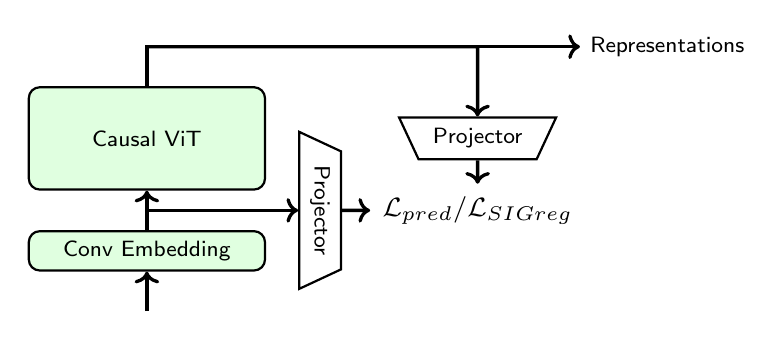
\begin{tikzpicture}[
      font=\sffamily\footnotesize,
      thick,
      mainbox/.style={
          draw,
          rounded corners,
          minimum width=3cm,
          minimum height=0.5cm,
          align=center,
          fill=green!12,
          anchor=south
      },
      trapezoidbox/.style={
          draw,
          trapezium,
          trapezium angle=65,
          minimum width=2cm,
          minimum height=0.5cm,
          fill=white,
          align=center
      },
      inputseqbox/.style={
          draw,
          minimum width=0.3cm,
          minimum height=0.6cm
      },
      seqbox/.style={
          draw,
          minimum width=0.9cm,
          minimum height=0.6cm
      },
      arrow/.style={->, line width=1.2pt}
  ]
      % --- Blocks ---
      \node[mainbox] (emb) at ($(0, 0.5)$) {Conv Embedding};
      \node[mainbox, minimum height=1.3cm] (pred) at ($(emb.north) + (0, 0.5)$) {Causal ViT};

      % --- Projectors ---
      \node[trapezoidbox, trapezium angle=-65] (pred_proj) at ($(pred) + (4.2, 0)$) {Projector};
      \node[trapezoidbox, rotate=-90] (target_proj) at ($(emb.north)!0.5!(pred.south) + (2.2, 0)$) {Projector};

      % --- Representations ---
      \node[anchor=west] (rep_lbl) at ($(pred.north) + (5.5, 0.5)$) {Representations};

      % --- Loss Function ---
      \node[scale=1.2] (loss) at (pred_proj |- target_proj) {$\mathcal{L}_{pred} / \mathcal{L}_{SIGreg}$};

      % --- Connections (arrows) ---
      \draw[arrow] (0, 0) -- (emb);
      \draw[arrow] (emb) -- (pred);

      \draw[arrow] (emb.north) |- (target_proj);
      \draw[arrow] (pred.north) |- (rep_lbl);
      \draw[arrow] (pred.north) |- (pred_proj |- rep_lbl) -- (pred_proj);

      \draw[arrow] (pred_proj) -- (loss);
      \draw[arrow] (target_proj) -- (loss);

  \end{tikzpicture}%
}
\caption{LeNEPA training diagram: the causal backbone predicts the next patch embedding; targets are aligned via the shifted regression objective in projected space. The projector is discarded during frozen-backbone evaluation.}
\Description{Block diagram of LeNEPA training. A time-series input is converted to convolutional patch embeddings, passed through a causal transformer, projected, and compared against shifted projected target embeddings using prediction and SIGReg losses.}
\label{fig:lenepa_tower}
\end{figure*}

\section{LeNEPA -- lean no-augmentation SSL architecture}
\label{sec:method_lenepa}

We introduce \textbf{Latent Euclidean Next-Embedding Prediction Architecture (LeNEPA)}, a lean no-augmentation Self-Supervised Learning (SSL) architecture based on Next-Embedding Prediction Architecture (NEPA)~\citep{xu2025nextembeddingprediction}.
We split the input data (univariate or multivariate time series) into a sequence of ViT-style patch embeddings with strided convolution and process the sequence with a causal transformer backbone~\citep{vaswani2017attention}.
LeNEPA learns by autoregressively predicting the next latent token: at each index $t$, it predicts a token and minimizes the mean squared error to the target at $t{+}1$.

Vanilla NEPA stabilizes training with a teacher network updated by an exponential moving average (EMA) and by blocking gradients through the targets; LeNEPA replaces this mechanism with \textbf{Sketched Isotropic Gaussian Regularization (SIGReg)}~\citep{balestriero2025lejepa}, which regularizes the token embedding distribution toward an isotropic Gaussian.
Following Guillotine Regularization~\citep{bordes2022guillotine}, we compute the prediction loss in a projected space and discard the projector at evaluation time.
Let $x\in\mathbb{R}^{B\times C\times L}$, let $z=\tau_{\theta}(x)\in\mathbb{R}^{B\times T\times D}$ be strided-convolution patch embeddings, and let $\hat z=f_{\phi}(z)$ be causal transformer outputs, where $\hat z_{b,t}$ depends only on $z_{b,1:t}$.
With projector $h_{\psi}:\mathbb{R}^{D}\rightarrow\mathbb{R}^{d}$, the LeNEPA prediction loss is
\begin{equation}
  \mathcal{L}_{\mathrm{pred}}
  =
  \frac{1}{B(T-1)}\sum_{b=1}^{B}\sum_{t=1}^{T-1}
  \left\|h_{\psi}(\hat z_{b,t}) - h_{\psi}(z_{b,t+1})\right\|_2^2 .
\label{eq:main_lenepa_pred}
\end{equation}
Unlike NEPA, LeNEPA does not stop gradients through the target tokens in Eq.~\eqref{eq:main_lenepa_pred}; stabilization comes from SIGReg.

For time series, global non-collapse is insufficient because tokens can also collapse along the temporal axis within each sample.
Let $u^{(\ell)}\in\mathbb{R}^{B\times T\times d}$ denote projected patch-token embeddings from layer $\ell$.
Unlike SIGReg regularization in the original LeJEPA design, we find that SIGReg over the temporal axis works best as a LeNEPA stabilizer: it regularizes the set of patch tokens within each sample,
\begin{equation}
  \mathcal{L}_{\mathrm{SIG}}^{\mathrm{time}}
  =
  \frac{1}{B|\mathcal{L}_{\mathrm{T}}|}\sum_{\ell\in\mathcal{L}_{\mathrm{T}}}\sum_{b=1}^{B}
  \mathrm{SIGReg}\!\left(\{u^{(\ell)}_{b,t}\}_{t=1}^{T}\right).
\label{eq:main_sigreg_time}
\end{equation}
The main objective is
\begin{equation}
  \mathcal{L}
  =
  \lambda_{\mathrm{pred}}\mathcal{L}_{\mathrm{pred}}
  +
  \lambda_{\mathrm{T}}\mathcal{L}_{\mathrm{SIG}}^{\mathrm{time}},
\label{eq:main_lenepa_objective}
\end{equation}
with $\lambda_{\mathrm{T}}=20$ and $\mathcal{L}_{\mathrm{T}}=\{0,8\}$ in the main PTB-XL/Aionoscope configuration;
this setting was selected from ablations run on PTB-XL (Table~\ref{tab:ablation_summary}).
We also evaluated batch-wise (B), pooled-representation (R), innovation/difference (I), and combined BRI placements; temporal (T) SIGReg was the only single-component placement with sustained frozen-backbone gains across both datasets.

\begin{lstlisting}[language=Python,caption={Compact LeNEPA training step},label={lst:main_lenepa_train}]
# x: [B, C, L]
z = patch_embed(x)                         # [B, T, D]
tokens = causal_transformer(z)              # list of per-layer [B, T, D]
z_hat = tokens[-1]                          # top-layer predictions

pred = projector(z_hat[:, :-1])
target = projector(z[:, 1:])                # no stop-gradient in LeNEPA
loss = lambda_pred * mse(pred, target)

u_T = [projector(tokens[l]) for l in sigreg_time_layers]
loss += lambda_T * SIGReg_time_per_sample(u_T)

loss.backward()
optimizer.step()
\end{lstlisting}

When evaluating frozen backbones, we find that intermediate layers provide stronger representations than the final layer for NEPA and LeNEPA (Section~\ref{sec:ablations_diagnostics}; Figure~\ref{fig:last_step_by_layer_lines}).
This is expected for next-embedding objectives: upper backbone blocks can partially act as an implicit predictor that maps features into the next-token regression space.
Therefore, we evaluate representations from all backbone layers and report results from the best-performing layer for each probe metric.

\section{Evaluation Protocol}
\label{sec:evaluation_protocol}

We evaluate representations with frozen-backbone probes because our goal is to test whether a pretraining recipe produces useful sequence embeddings when reused unchanged.
Throughout the paper, \textbf{LeNEPA} denotes the objective and architecture, not a single shared checkpoint or foundation encoder.
We use three separately pretrained LeNEPA encoders: \textbf{LeNEPA-PTBXL}, trained on PTB-XL~\citep{wagner2020ptbxl}; \textbf{LeNEPA-Aionoscope}, trained on Aionoscope; and \textbf{LeNEPA-CauKer}, trained on CauKer~\citep{xie2025cauker}.
These checkpoints share the same no-augmentation latent-prediction recipe, but their weights are trained independently.

We separate two evaluation questions to avoid conflating recipe reuse with checkpoint transfer.
\textbf{Fixed-recipe pretraining reuse} asks whether the same SSL objective configuration can be reused when the pretraining distribution changes, without re-designing method-specific augmentations or loss hyperparameters.
We test this by training both methods independently on both datasets: LeNEPA-PTBXL and LeNEPA-Aionoscope use exactly the same no-augmentation objective configuration, while JEPA-PTBXL and JEPA-Aionoscope use the same ECG-tuned view recipe. In both cases, only the pretraining dataset changes.
Crucially, both recipes were developed and fixed using PTB-XL experiments: the JEPA masking schedule was tuned for ECG morphology, and the LeNEPA SIGReg configuration ($\lambda_{\mathrm{T}}=20$, layers $\{0,8\}$) was likewise selected from PTB-XL ablations.
Neither recipe was optimized for Aionoscope.
We hypothesize that masking recipes encode domain-semantic assumptions---which temporal regions constitute meaningful prediction targets---whereas regularization hyperparameters primarily encode optimization dynamics; moving from a masking-based view recipe to an augmentation-free regularization-based recipe should therefore reduce the domain-specific tuning required when the signal family changes.
This protocol does not test the best possible Aionoscope-tuned JEPA configuration; a JEPA recipe designed for Aionoscope's signal characteristics would likely recover strong performance. Rather, the experiment measures the cost of relying on ECG-masking assumptions when that recipe is reused on a structurally different signal family.
\textbf{Frozen-encoder checking} asks whether one pretrained encoder can produce useful features on new downstream datasets without changing its weights.
We test this by training LeNEPA-CauKer once, freezing it, extracting per-layer embeddings, and evaluating Random-Forest probes on UCR-128, following the MantisV2 testing protocol~\citep{feofanov2026mantisv2}.

\begin{table}[t]
\centering
\caption{Pretrained encoder instances used in the evaluation. Each row is a separately pretrained checkpoint.}
\label{tab:lenepa_instances}
\small
\setlength{\tabcolsep}{3pt}
\begin{tabularx}{\linewidth}{l X X X}
\toprule
Encoder & Pretraining & Evaluation & Purpose \\
\midrule
LeNEPA-PTBXL
  & PTB-XL
  & PTB-XL
  & In-domain ECG reference against ECG-tuned JEPA \\
LeNEPA-Aionoscope
  & Aionoscope
  & Aionoscope
  & Fixed-recipe reuse across signal families \\
JEPA-PTBXL
  & PTB-XL
  & PTB-XL
  & ECG-tuned JEPA reference under the same fixed-horizon protocol \\
JEPA-Aionoscope
  & Aionoscope
  & Aionoscope
  & Same ECG-tuned JEPA recipe retrained on Aionoscope to test unchanged reuse \\
LeNEPA-CauKer
  & CauKer
  & UCR-128
  & Frozen-encoder check on external classification datasets \\
\bottomrule
\end{tabularx}
\end{table}

Table~\ref{tab:reproducibility_config} summarizes the configuration used for the headline experiments.
Full training, evaluation, and plotting code together with exact configuration files will be released under an open-source license; Table~\ref{tab:reproducibility_config} and Listing~\ref{lst:main_lenepa_train} provide the information needed to reproduce the headline experiments.

\begin{table*}[t]
\centering
\scriptsize
\caption{Implementation and evaluation configuration for the main experiments. PTB-XL and Aionoscope use the same fixed-horizon recipe-reuse matrix; the CauKer/UCR row documents the frozen-encoder check in Table~\ref{tab:ucr_mantis_comparison}.}
\label{tab:reproducibility_config}
\setlength{\tabcolsep}{3pt}
\begin{tabularx}{\textwidth}{p{0.16\textwidth} X X}
\toprule
Item & PTB-XL / Aionoscope fixed-horizon matrix & CauKer $\rightarrow$ UCR-128 frozen-encoder check \\
\midrule
Training horizon and seeds
& $20{,}000$ gradient steps; seeds $s\in\{0,1,2,3,4\}$; offline probes every $1{,}000$ steps, including step $0$
& $20{,}000$ gradient steps; seed $0$; UCR evaluated at each saved checkpoint and reported at the best and final checkpoints \\
Optimizer
& AdamW, batch size $256$, bfloat16; cosine learning-rate schedule $10^{-4}\rightarrow10^{-6}$ with $1{,}000$ warmup steps; weight decay $0.01\rightarrow0.1$; betas $(0.9,0.99)$
& AdamW, batch size $256$, bfloat16; cosine learning-rate schedule $2{\times}10^{-4}\rightarrow2{\times}10^{-4}$ with $1{,}000$ warmup steps; weight decay $0.01\rightarrow0.1$; betas $(0.9,0.99)$ \\
Backbone and tokenizer
& Causal ViT-XS, depth $8$, $4$ heads, MLP ratio $4$, QK-Norm $(\epsilon=10^{-6})$, SwiGLU, RoPE; Conv1d patch embedding with $P=25$ for length-$5000$ signals; $D=192$; mean-pooling readout
& Causal ViT-XS, depth $8$, $4$ heads, MLP ratio $4$, QK-Norm, SwiGLU, RoPE; length-$5000$ CauKer sequences; $D=256$; sequence-normalized scalar-statistics path added for the Mantis-facing UCR comparison \\
LeNEPA loss
& Projected MSE next-token loss, no stop-gradient, $\lambda_{\mathrm{pred}}=1$; temporal SIGReg with $\lambda_{\mathrm{T}}=20$ on layers $\{0,8\}$; projector is MLP+BN+ReLU with output dimension $64$
& Same projected next-token objective; temporal SIGReg on layers $\{0,8\}$ with $\lambda_{\mathrm{T}}=2.5$; projector output dimension $64$ \\
JEPA view recipe
& Fixed ECG-tuned masking view recipe with keep ratio $\rho\sim\mathrm{Uniform}(0.15,0.25)$; JEPA evaluated with both CLS-token and mean-pooling readouts
& Not used \\
Probe protocol
& Frozen per-layer linear probes on layers $0$--$8$; $5{,}000$ probe steps; AdamW, learning rate $0.01$, weight decay $0$, batch size $256$; metrics aggregated as median and sample standard deviation across seeds
& Frozen per-layer embeddings on UCR-128; Random Forest classifier with $200$ trees and all 128 train/test splits; mean accuracy averaged across datasets \\
\bottomrule
\end{tabularx}
\end{table*}

For the NEPA/LeNEPA/JEPA comparisons on PTB-XL and Aionoscope, all methods use the same ViT-XS backbone size and are trained for a fixed horizon of $20{,}000$ gradient steps.
For NEPA/LeNEPA, we use mean pooling over causal patch-token representations; for JEPA, we report both CLS-token and mean-pooling readouts to control for readout mismatch.
Because next-embedding objectives can place the most probe-useful representation at an intermediate depth, we train offline linear probes on frozen per-layer representations for layers $0$--$8$.
For the last-step headline LeNEPA classification readouts, we use a fixed mid-layer $L4$ representation rather than an oracle layer; this is conservative on PTB-XL and exactly matches the best layer on Aionoscope and the best UCR checkpoint (Table~\ref{tab:layer_selection_sensitivity}).
For JEPA/NEPA baselines and dense Aionoscope diagnostics, we retain best-layer values to avoid penalizing baselines for their different depth profiles and to keep dense probes as diagnostic rather than headline comparison metrics.
We evaluate probes every $1{,}000$ pretraining steps, including step $0$, and report last-step values unless stated otherwise.
For PTB-XL and Aionoscope, each objective--dataset pair is repeated with five random seeds; tables and plots in this paper aggregate per-seed metrics as median $\pm$ sample standard deviation.
For delta summaries, we compute each seed's difference between step $20{,}000$ and step $0$, selecting the best layer independently at each step.
For early-gain summaries on AUROC/AUPRC, define the normalized gain
\begin{equation}
  r_m(t)=\frac{m(t)-m(0)}{m(20{,}000)-m(0)}
\end{equation}
for metric $m$ at pretraining step $t$, and let $\tau_q(m)$ be the first offline-probe evaluation step at which $r_m(t)\ge q$.
We compute these thresholds on the median learning curves in Figure~\ref{fig:dynamics_best_layer_classification_transfer}; because probes are evaluated every $1{,}000$ steps, $\tau_q$ is a discrete step count rather than an interpolated time.

PTB-XL is a 12-lead ECG classification dataset with clinically meaningful multi-label targets~\citep{wagner2020ptbxl}.
This benchmark is a useful in-domain test because ECG\_JEPA is a strong baseline designed around ECG-specific JEPA augmentations~\citep{weimann2024jepaecg}.
To test fixed-recipe reuse across a different signal family, we use \textbf{Aionoscope}, implemented as an online generator rather than a fixed finite dataset.
In this paper we use Aionoscope as a controlled pretraining and frozen-probe benchmark.
The stream used here is a basic-components generator of univariate sequences of length $5000$.
Each sample is generated by selecting $2$ active latent components from a fixed inventory of $14$ component types spanning constant baselines, noise processes, trends, periodic waveforms, and sparse events.
The main stream is intentionally imbalanced: most components have sampling weight $1.0$, while six rare components have weight $0.02$ (\texttt{gaussian\_noise}, \texttt{log\_trend}, \texttt{square}, \texttt{spike}, \texttt{level\_change}, and \texttt{gaussian}).

Aionoscope exposes two kinds of targets used for frozen-backbone probing.
Categorical targets are multi-hot indicators of the active component types and are evaluated with macro AUROC/AUPRC.
Dense targets are scalar generative parameters recorded by the generator metadata, including noise scale, trend coefficients, periodic amplitude/frequency/phase/offset, and event time/amplitude/width; disabled components are masked for the corresponding dense target.
SSL training never uses these targets.
Pretraining and probing streams use separate fixed RNG streams, so probes evaluate fresh generated samples from the same distribution rather than memorized training examples.

Finally, we include a frozen-encoder check by testing LeNEPA-CauKer trained on CauKer~\citep{xie2025cauker} on the full UCR archive of 128 univariate classification datasets~\citep{dau2019ucr}.
Unlike the PTB-XL/Aionoscope fixed-recipe study, the CauKer-to-UCR experiment evaluates a single frozen LeNEPA checkpoint across 128 external datasets.
For this experiment, we follow the Mantis frozen-feature protocol: extract frozen per-layer sequence embeddings, train a Random Forest classifier on each dataset's training split, evaluate on its test split, and average accuracy across datasets~\citep{feofanov2026mantisv2,xie2025cauker}.
We use the original Mantis Random-Forest result as the primary published anchor, and report NuTime and MOMENT only as protocol-matched context from the MantisV2 Random-Forest comparison~\citep{lin2024nutime,goswami2024moment}.

\begin{figure*}[t]
\centering
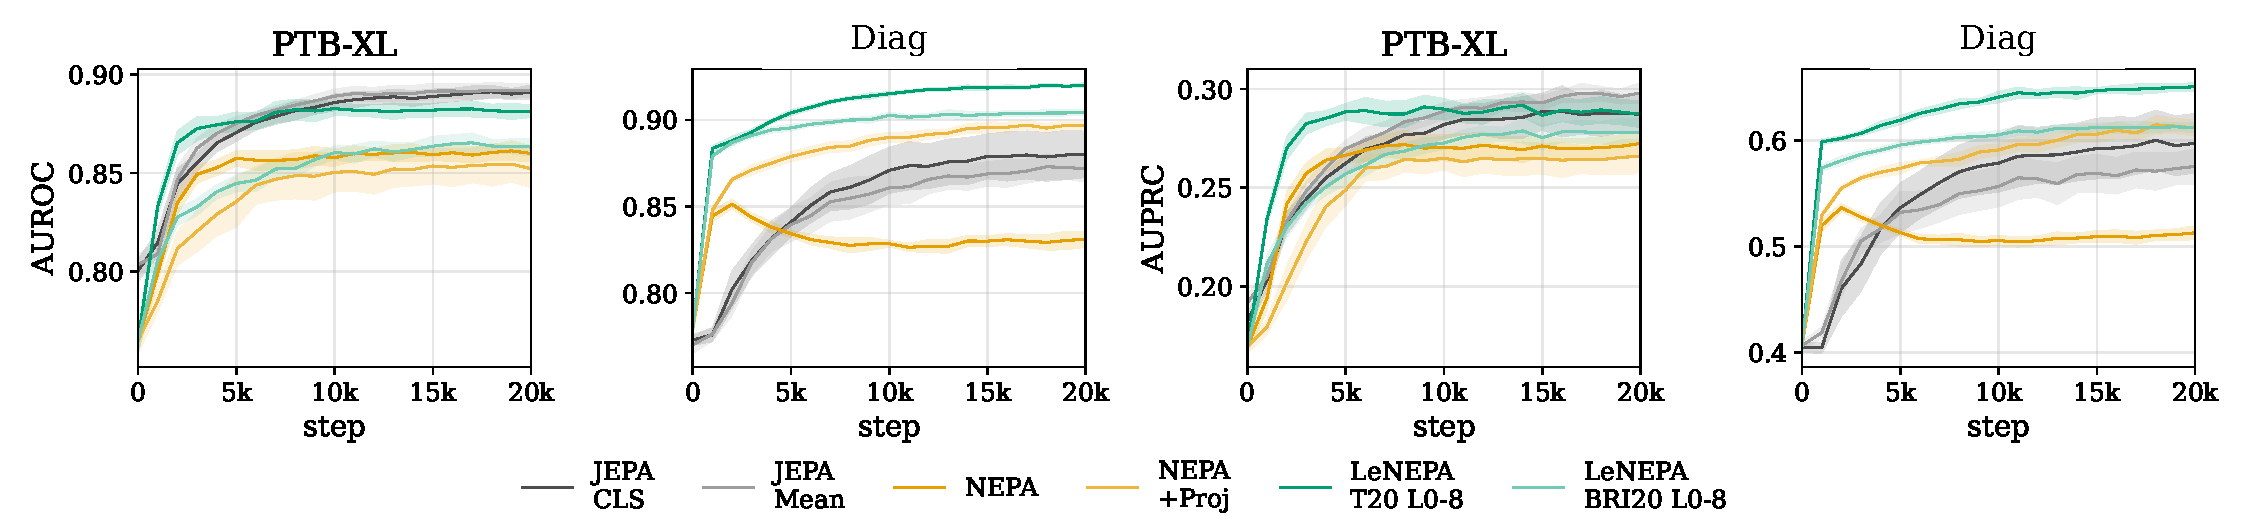
\includegraphics[width=\textwidth]{figures/dynamics_best_layer_classification_transfer.pdf}
\caption{PTB-XL/Aionoscope fixed-recipe reuse experiment: best-layer frozen-backbone classification dynamics over the fixed $20{,}000$-step pretraining horizon. Curves show AUROC/AUPRC at each offline-probe evaluation step for PTB-XL and Aionoscope. This tests recipe portability, not shared-checkpoint transfer or a claim that Aionoscope-tuned JEPA cannot work. Both methods are trained separately on each dataset; the fixed ECG-tuned JEPA recipe remains strong in-domain but is weaker when reused unchanged on Aionoscope.}
\Description{Four line plots showing AUROC and AUPRC over pretraining steps for PTB-XL and Aionoscope. LeNEPA improves rapidly and remains strong on Aionoscope, while the ECG-tuned JEPA recipe has weaker gains when reused unchanged on Aionoscope.}
\label{fig:dynamics_best_layer_classification_transfer}
\end{figure*}

\begin{table*}[t]
\centering
\small
\caption{PTB-XL/Aionoscope fixed-horizon experiment matrix at the last step ($20{,}000$ updates) for the controlled five-seed comparisons. JEPA/NEPA rows report best-layer frozen-backbone probes; LeNEPA classification columns use a fixed $L4$ readout, while LeNEPA dense Aionoscope columns report metric-specific best-layer diagnostic probes. Values are aggregated across seeds as $\mathrm{median}(\mathrm{std})$, with std shown in $10^{-3}$ units.}
\label{tab:summary_selected_best_last_step}
\begin{tabular*}{\textwidth}{@{\extracolsep{\fill}}llcccccccc@{}}
\toprule
\multicolumn{2}{c}{} & \multicolumn{2}{c}{PTB-XL} & \multicolumn{6}{c}{Aionoscope} \\
\cmidrule(lr){3-4} \cmidrule(lr){5-10}
model & config & \multicolumn{1}{c}{AUROC $\uparrow$} & \multicolumn{1}{c}{AUPRC $\uparrow$} & \multicolumn{1}{c}{AUROC $\uparrow$} & \multicolumn{1}{c}{AUPRC $\uparrow$} & \multicolumn{1}{c}{MSE $\downarrow$} & \multicolumn{1}{c}{MAE $\downarrow$} & \multicolumn{1}{c}{Pearson $\uparrow$} & \multicolumn{1}{c}{$R^2$ $\uparrow$} \\
\midrule
JEPA & CLS & \textbf{0.891(3)} & \underline{0.287(9)} & 0.880(13) & 0.597(28) & 1.065(13) & 0.515(5) & 0.480(12) & -0.005(24) \\
JEPA & Mean & \textbf{0.892(3)} & \textbf{0.298(5)} & 0.872(7) & 0.576(16) & 1.113(13) & 0.548(5) & 0.462(11) & -0.514(291) \\
NEPA &  & 0.860(3) & 0.272(5) & 0.831(4) & 0.513(6) & 1.001(9) & 0.461(3) & 0.522(4) & \underline{0.197(24)} \\
NEPA & +Proj & 0.852(9) & 0.266(8) & \underline{0.897(2)} & \underline{0.612(7)} & \underline{0.827(8)} & \textbf{0.382(3)} & \textbf{0.610(7)} & \textbf{0.348(23)} \\
LeNEPA & T20 L0-8 & \underline{0.880(6)} & \underline{0.285(5)} & \textbf{0.920(1)} & \textbf{0.650(4)} & \textbf{0.797(12)} & \underline{0.405(4)} & \underline{0.584(6)} & 0.164(105) \\
\bottomrule
\end{tabular*}
\end{table*}


\begin{table*}[t]
\centering
\caption{UCR-128 frozen-encoder check. We report mean accuracy over all 128 UCR datasets using frozen sequence embeddings and a Random Forest classifier. The table lists each model's pretraining data because baselines differ in architecture, objective, and whether UCR/UEA training data or larger heterogeneous corpora were used. The LeNEPA-CauKer row reports the best checkpoint over the fixed $20{,}000$-step trajectory; Mantis is the closest published CauKer-only Mantis-family anchor, and NuTime/MOMENT provide protocol-matched context from the same Random-Forest comparison.}
\label{tab:ucr_mantis_comparison}
\small
\setlength{\tabcolsep}{3pt}
\begin{tabularx}{\textwidth}{l X l l X X r}
\toprule
Model & Pretrain data & Params & Attention & Tokenizer / input engineering & SSL objective & Acc. (\%) \\
\midrule
LeNEPA
  & CauKer; no UCR
  & $6.3$M
  & causal
  & Conv patches + global stats
  & latent prediction; no aug.
  & $\mathbf{77.65}$ \\
Mantis
  & CauKer; no UCR
  & $8.1$M
  & bidirectional
  & Conv patches + patch stats + diff
  & contrastive; crop aug.
  & $78.81$ \\
NuTime~\citep{lin2024nutime}
  & incl. UCR/UEA train
  & $2.0$M
  & bidirectional
  & Window shape + window stats
  & BYOL; crop aug.
  & $77.32$ \\
MOMENT~\citep{goswami2024moment}
  & incl. UCR/UEA train
  & $161$M
  & bidirectional
  & T5 patches
  & masked reconstruction
  & $77.89$ \\
\bottomrule
\end{tabularx}
\vspace{0.25em}
\footnotesize
LeNEPA-CauKer peaks at $77.65\%$ at $17{,}000$ steps and remains at $77.20\%$ at the final $20{,}000$-step checkpoint (Figure~\ref{fig:ucr_layer_profile_lenepa_seqnorm}).
LeNEPA-CauKer row adds MSSE for this Mantis-facing UCR comparison because Mantis itself uses an MSSE-encoded scalar-statistics path; the main LeNEPA experiments elsewhere in the paper do not rely on MSSE.
NuTime/MOMENT entries use the Random-Forest UCR-128 averages reported in MantisV2~\citep{feofanov2026mantisv2}.
\end{table*}

\section{Experiments}
\label{sec:experiments}

\begin{figure}[t]
\centering
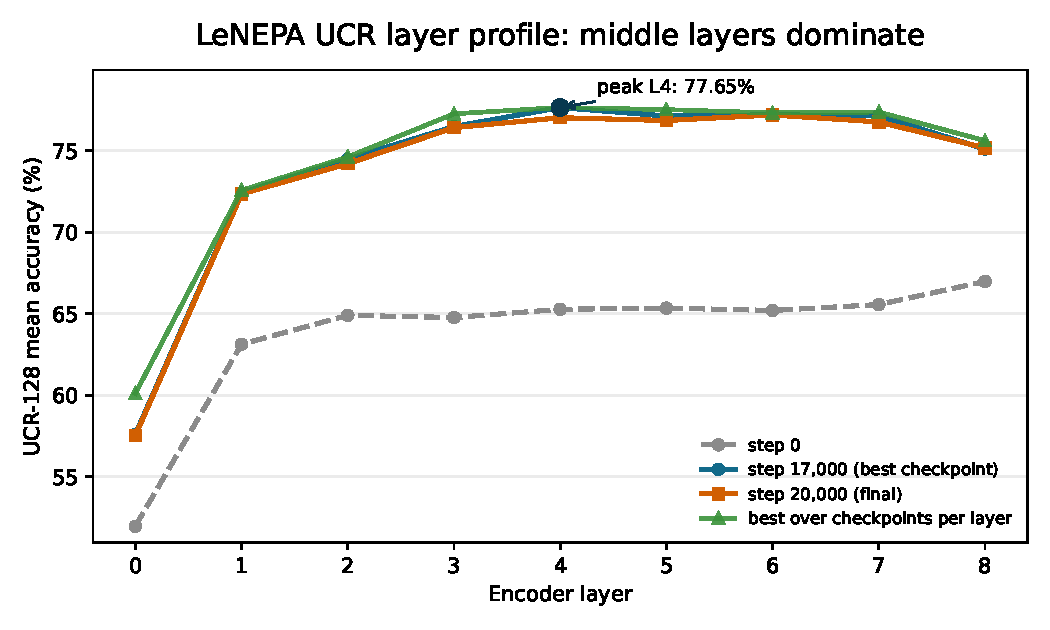
\includegraphics[width=\linewidth]{figures/ucr_layer_profile_lenepa_seqnorm.pdf}
\caption{UCR-128 layer-profile diagnostic for the LeNEPA-CauKer run used in Table~\ref{tab:ucr_mantis_comparison}. Each point is mean Random-Forest accuracy over the 128 UCR datasets for one frozen backbone layer. Intermediate layers outperform the final layer: the run peaks at $77.65\%$ at $17{,}000$ steps ($L4$) and remains at $77.20\%$ at the final $20{,}000$-step checkpoint ($L6$).}
\Description{Line plot of UCR-128 Random Forest accuracy by LeNEPA layer for selected checkpoints. Intermediate layers peak above the final layer.}
\label{fig:ucr_layer_profile_lenepa_seqnorm}
\end{figure}

We evaluate frozen-backbone representations using per-layer probes.
For time series, we evaluate fixed-recipe reuse on PTB-XL (12-lead ECG classification) and Aionoscope (classification + dense regression), then use UCR-128 as a separate frozen-encoder check.

\paragraph{Fixed-recipe reuse: PTB-XL vs. Aionoscope.}
The baseline JEPA model~\citep{weimann2024jepaecg} is tuned for ECG and relies on dataset-specific augmentations, and thus performs well on the dataset it was designed for.
In this in-domain regime, LeNEPA remains competitive, showing that eliminating augmentations does not preclude useful frozen features.
We then test fixed-recipe reuse by training both LeNEPA and JEPA again on Aionoscope while keeping each method's recipe unchanged.
As shown by Figure~\ref{fig:dynamics_best_layer_classification_transfer}, the JEPA configuration that is strong on PTB-XL is weaker when reused unchanged on Aionoscope: JEPA-Aionoscope's training gains shrink markedly, whereas LeNEPA-Aionoscope retains strong training gains and beats JEPA-Aionoscope both in final performance and training dynamics.
This does not rule out an Aionoscope-tuned JEPA recipe; a JEPA recipe designed for Aionoscope's signal characteristics would likely recover competitive performance. Rather, the experiment identifies \emph{ECG-masking assumptions}---the semantic tie between JEPA's view recipe and ECG morphology---as a source of fragility when that recipe is reused on a structurally different signal family.
A general-purpose JEPA masking recipe might transfer better, but would still require per-domain view engineering: exactly the cost that a no-augmentation objective avoids by design.
Finally, Figure~\ref{fig:dynamics_best_layer_classification_transfer} summarizes early learning dynamics under the time-to-gain definition in Section~\ref{sec:evaluation_protocol}.
On the median AUROC/AUPRC curves, LeNEPA reaches $80\%$ of its final gain after $2$--$5$k updates across PTB-XL and Aionoscope, whereas the faster JEPA readout reaches the same threshold after $5$--$10$k updates; because probes are evaluated every $1{,}000$ steps these thresholds are coarse discrete counts and per-seed timing varies.
The $90\%$ threshold is less uniform---LeNEPA reaches it after $5$--$10$k updates, while JEPA typically reaches it after $10$--$15$k updates---so we interpret these observations as qualitative evidence of faster early representation acquisition in this fixed-recipe protocol.

\paragraph{Frozen-encoder check: CauKer to UCR-128.}
We use UCR-128 as a frozen-encoder check that complements the fixed-recipe reuse study. We choose Mantis as the primary comparator because it is a state-of-the-art SSL/foundation architecture for time-series classification and is close to LeNEPA in the relevant evaluation regime: a frozen time-series encoder followed by a lightweight classifier~\citep{feofanov2025mantis,feofanov2026mantisv2}.
UCR-128 classification accuracy is Mantis's headline contribution; its architecture was purpose-built for this setting: bidirectional attention (full sequence context), a handcrafted first-difference branch, and a contrastive objective with Random Crop Resize augmentations.
The closest published anchor from this architecture uses frozen Mantis representations and reports $78.81\%$ average accuracy on all 128 UCR datasets with a Random Forest classifier.
As shown in Table~\ref{tab:ucr_mantis_comparison}, our LeNEPA-CauKer run peaks at $77.65\%$ over the fixed $20$k-step pretraining trajectory (single seed) and remains at $77.20\%$ at the final checkpoint (Figure~\ref{fig:ucr_layer_profile_lenepa_seqnorm}).
We treat this single-seed result as an existence proof: a LeNEPA encoder with causal attention, no augmentations, and no first-difference branch---each a structural disadvantage relative to Mantis for UCR classification---can already produce frozen features competitive with a model that was specifically designed and optimised for this benchmark.
Additional seeds would characterise variance; this run establishes that the no-augmentation causal recipe can reach the Mantis neighbourhood without any UCR-specific engineering.
NuTime and MOMENT in the same MantisV2 Random-Forest UCR table are reported as $77.32\%$ and $77.89\%$, respectively; the best LeNEPA checkpoint is above NuTime and within $0.24$ percentage points of MOMENT~\citep{lin2024nutime,goswami2024moment}.
Because this comparison uses a single LeNEPA pretraining seed, a best checkpoint over the trajectory, and baselines with different pretraining corpora and architectures, we treat it as protocol-matched context for the frozen features.
We therefore do not treat stronger MantisV2 final-comparison or leaderboard numbers as direct baselines, because they are designed for leaderboard performance through heavier model and test-time/evaluation choices rather than for isolating the effect of a no-augmentation objective.

The following diagnostics summarize the main ablations needed to interpret the results.

\section{Ablations and Diagnostics}
\label{sec:ablations_diagnostics}

Aionoscope acts as diagnostic instrumentation rather than as a paper contribution.
Each generated sequence has known latent factors and categorical/dense targets; SSL pretraining does not use these labels, and they are used only after freezing the backbone to probe which factors are linearly recoverable from each layer.

Table~\ref{tab:ablation_summary} summarizes the controlled ablations behind the main LeNEPA design choices.
Because the page limit prevents full ablation tables, we report the design-level conclusions here.
The projector rows test the Guillotine Regularization idea that SSL losses can be applied in a disposable head while evaluating the truncated backbone~\citep{bordes2022guillotine}.
As Table~\ref{tab:summary_selected_best_last_step} shows, NEPA with a projector (NEPA\,+\,Proj) is already a strong baseline: it outperforms LeNEPA on several dense Aionoscope metrics (MAE, Pearson, $R^2$) while LeNEPA leads on classification (AUROC, AUPRC) and MSE.
The contribution of temporal SIGReg over NEPA\,+\,Proj is therefore most clearly visible on classification and training dynamics, while the dense regression picture is more mixed.

\begin{table*}[t]
\centering
\small
\caption{Compact ablation summary supporting the LeNEPA design choices.}
\label{tab:ablation_summary}
\setlength{\tabcolsep}{4pt}
\renewcommand{\arraystretch}{1.12}
\begin{tabularx}{\textwidth}{p{0.18\textwidth} p{0.30\textwidth} p{0.25\textwidth} X}
\toprule
Design question & Controlled ablation & Main observation & Implication \\
\midrule
Projector loss space
& Guillotine-style projector: NEPA/LeNEPA trained with and without the projector
& Projector-enabled variants improve $22/24$ last-step probe comparisons.
& Compute prediction and SIGReg losses in projected space, then discard the projector for evaluation. \\
\addlinespace
Projector capacity
& Output width, hidden width, and MLP depth of the Guillotine-style projector
& Larger or deeper projectors do not improve performance over the fixed projector used in the main runs.
& The main projector effect comes from separating the loss space from the evaluated backbone space, not from adding projector capacity. \\
\addlinespace
SIGReg axis
& Temporal (T) SIGReg versus batch-wise (B), pooled-representation (R), innovation/difference (I), and batch-time (BT) placements
& Temporal SIGReg is the only single-component placement with sustained frozen-backbone gains across PTB-XL and Aionoscope.
& Use Temporal SIGReg as the LeNEPA anti-collapse stabilizer. \\
\addlinespace
SIGReg layer placement
& Temporal SIGReg on both prediction/target sides $\{0,8\}$ vs.\ one side or inner layers
& Regularizing both sides of the prediction relation is more stable in our fixed-recipe runs; target-only or off-path regularization can degrade or collapse.
& Apply SIGReg where it directly counterbalances the next-embedding prediction loss. \\
\addlinespace
JEPA view recipe
& PTB-XL JEPA keep-ratio $(0.15,0.25)$ vs.\ $(0.05,0.10)$ and $(0.30,0.40)$
& A $2$--$3\times$ change in masking strength substantially degrades probe dynamics.
& Augmentation/view hyperparameters can be sensitive, motivating a no-augmentation objective. \\
\bottomrule
\end{tabularx}
\end{table*}

Finally, layer-wise probing reveals a pattern that is increasingly important for latent-prediction encoders.
Across both datasets, JEPA probe performance tends to improve with depth and peak near the top layers.
In contrast, NEPA and LeNEPA often achieve their best probe scores at intermediate layers (frequently around $l\approx3$--$5$), with the final layer sometimes underperforming these mid-level representations.
This suggests that the deepest blocks of next-embedding predictors can partially specialize to the prediction task, while intermediate layers retain more probe-useful features.

\paragraph{Layer-selection sensitivity.}
The best-layer protocol is an oracle upper bound.
The key question is therefore whether this oracle choice materially changes the conclusions.
We check this by comparing oracle selection to a fixed mid-layer readout.
Table~\ref{tab:layer_selection_sensitivity} compares the oracle best layer with a fixed $L4$ readout and the final transformer layer $L8$ for LeNEPA classification results.
The classification optima are concentrated in the middle of the backbone: PTB-XL peaks at $L5$, while Aionoscope and the best UCR checkpoint peak at $L4$.
Across the five-seed PTB-XL and five-seed Aionoscope classification evaluations, using the fixed $L4$ readout removes almost all of the oracle advantage, whereas using the final layer can be substantially worse.
Thus, the LeNEPA classification conclusions do not rely on per-dataset layer tuning; dense Aionoscope probes are more metric-dependent and should be read primarily as diagnostics of where information appears in the backbone.

\begin{table}[t]
\centering
\scriptsize
\caption{Layer-selection sensitivity motivating the fixed-$L4$ LeNEPA classification readout. Best-layer values are oracle selections over probed layers; fixed $L4$ uses one mid-layer readout across datasets; $L8$ is the final transformer layer. Parentheses report the difference from the oracle value.}
\label{tab:layer_selection_sensitivity}
\begin{tabular}{llrrrr}
\toprule
Dataset & Metric & Oracle layer & Oracle & Fixed $L4$ ($\Delta$) & Final $L8$ ($\Delta$) \\
\midrule
PTB-XL & AUROC & $L5$ & $0.880$ & $0.880$ ($0.000$) & $0.835$ ($-0.045$) \\
PTB-XL & AUPRC & $L5$ & $0.287$ & $0.285$ ($-0.002$) & $0.203$ ($-0.084$) \\
Aionoscope & AUROC & $L4$ & $0.920$ & $0.920$ ($0.000$) & $0.895$ ($-0.025$) \\
Aionoscope & AUPRC & $L4$ & $0.650$ & $0.650$ ($0.000$) & $0.607$ ($-0.043$) \\
UCR-128 & Accuracy & $L4$ & $77.65$ & $77.65$ ($0.00$) & $75.10$ ($-2.55$) \\
\bottomrule
\end{tabular}
\end{table}

\begin{figure*}[p]
\centering
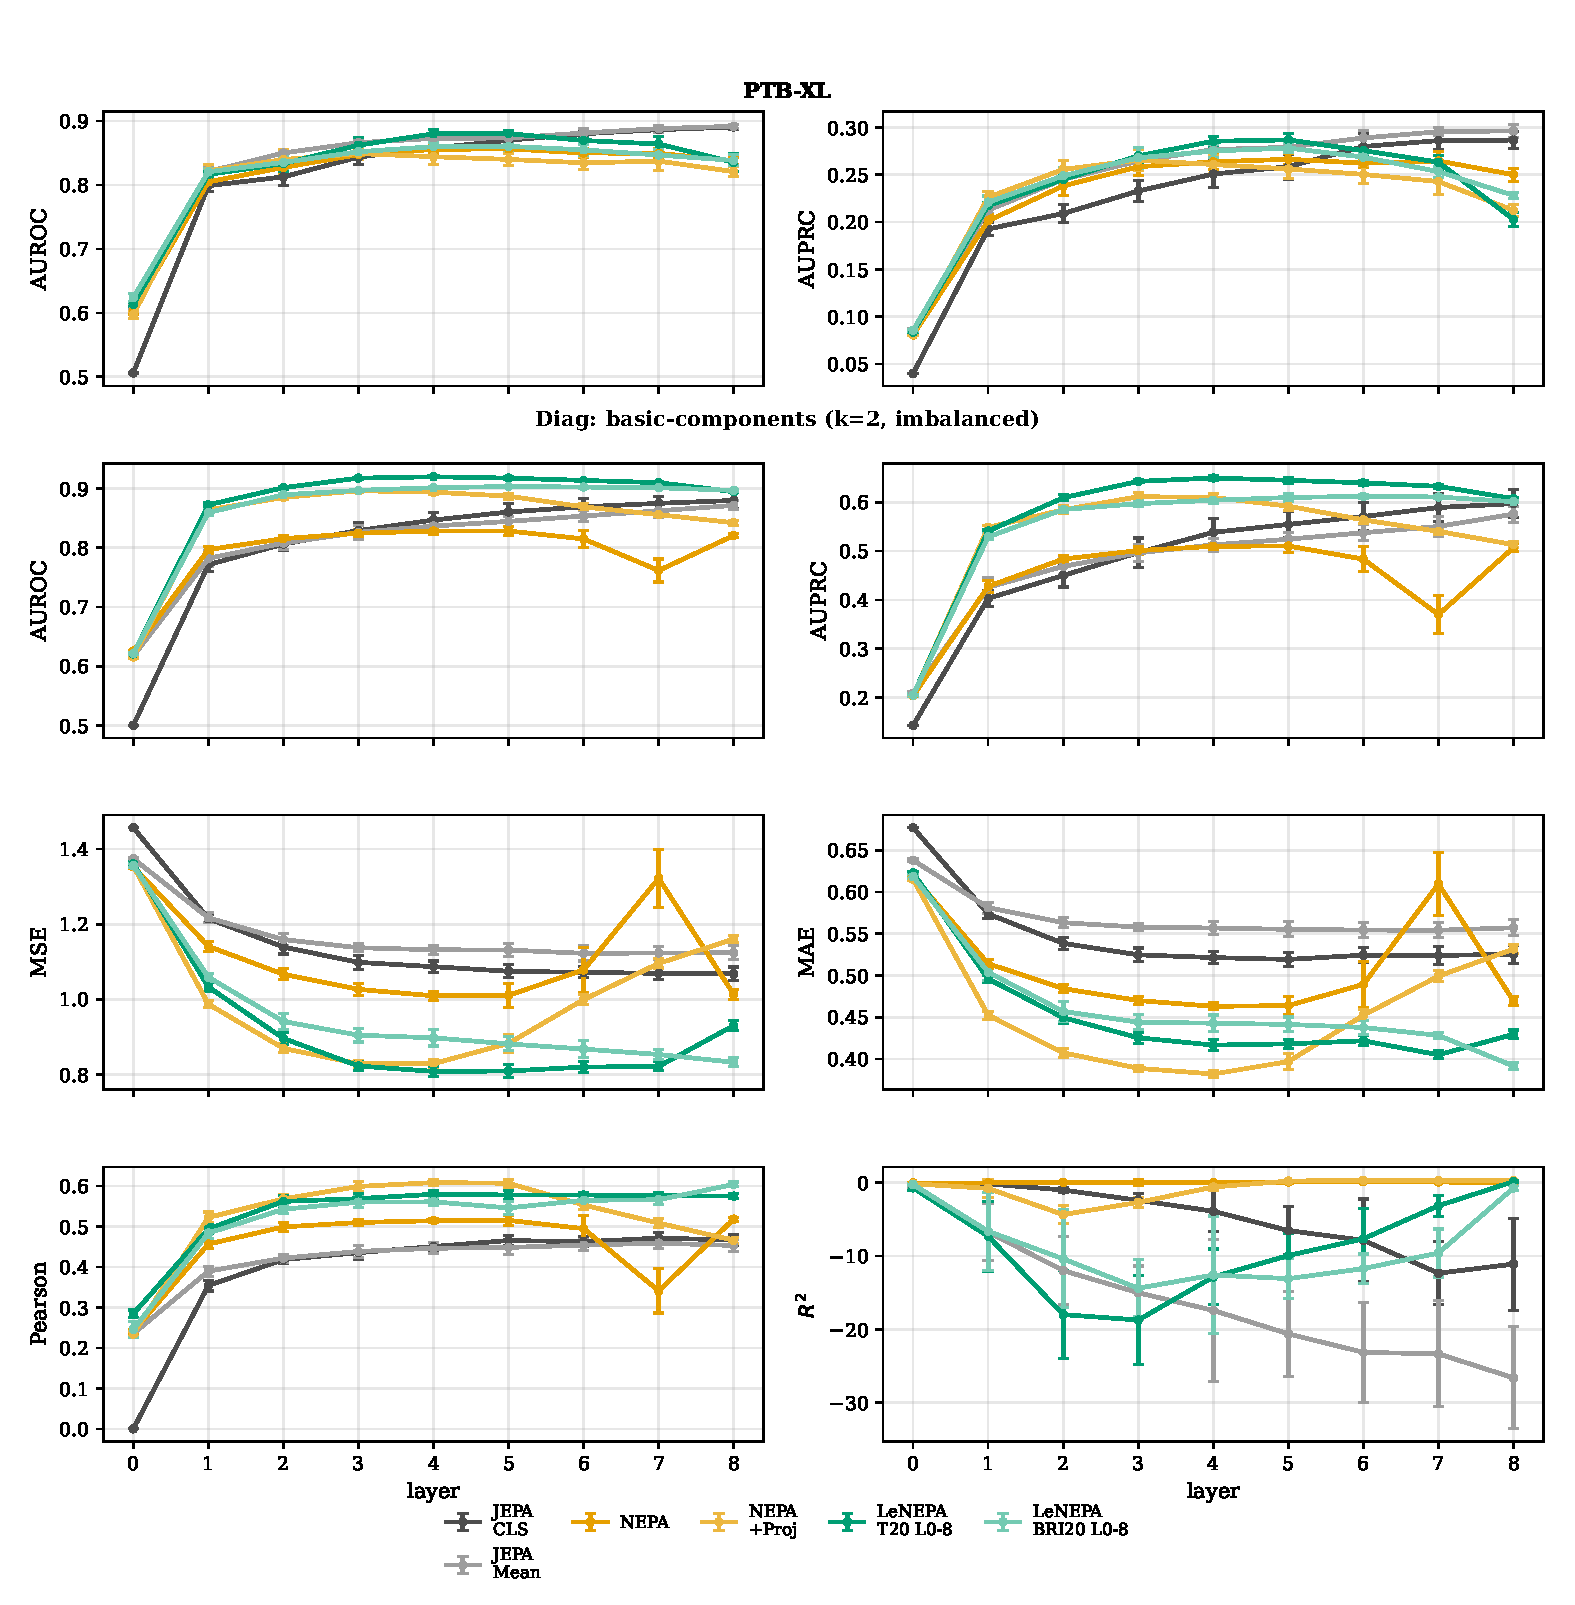
\includegraphics[width=\textwidth]{figures/last_step_by_layer_lines.pdf}
\caption{Last-step (step $20{,}000$) layer-wise frozen-backbone probe results. We report PTB-XL (top row; AUROC/AUPRC) and Aionoscope \emph{basic-components} results (bottom rows; AUROC/AUPRC and MSE/MAE/Pearson/$R^2$). Each line corresponds to a method; points denote probed layers $0$--$8$.}
\Description{Line plots of frozen-backbone probe performance across backbone layers for PTB-XL and Aionoscope diagnostic metrics.}
\label{fig:last_step_by_layer_lines}
\end{figure*}

\section{Limitations and Future Work}
\label{sec:limitations}

While LeNEPA removes one source of time-series SSL engineering by avoiding augmentations, our current study tests recipe portability rather than claiming a foundation encoder.
The convolutional tokenizer still depends on dataset-specific design choices such as kernel size and stride, implicitly assumes regular sampling, and may limit transfer across signals with different temporal scales.
Although the PTB-XL/Aionoscope fixed-recipe runs use the same temporal SIGReg setting, SIGReg still introduces scale and placement hyperparameters; the CauKer/UCR run uses a smaller temporal scale in a different tokenizer configuration, so principled defaults across dataset scales and tokenizers remain future work.
Aionoscope is also a synthetic diagnostic benchmark whose full specification is outside the scope of this paper.
Some diagnostic analyses and baseline comparisons still report best-layer values; those should be treated as oracle upper bounds unless a layer is fixed a priori or selected using labeled validation data.
For LeNEPA classification, the reported last-step readout is fixed to $L4$ and is stable relative to the oracle choice (Table~\ref{tab:layer_selection_sensitivity}).
The UCR-128 frozen-encoder check broadens the evidence beyond PTB-XL and Aionoscope, but it is still univariate and uses one pretraining seed; broader UEA-style multivariate evaluations remain necessary.

\section{Conclusion}
\label{sec:conclusion}

Time-series SSL recipes are often entangled with view and augmentation choices that may be safe in one signal family but mismatched in another.
We studied this issue as a \emph{fixed-recipe stress test}: keep each method's SSL recipe unchanged, retrain on a new pretraining distribution, and evaluate whether frozen representations remain useful.
This setting is intentionally narrower than fully tuned benchmark comparison; it measures the cost of recipe reuse, not the best attainable performance after retuning.

We proposed \textbf{LeNEPA}, a no-augmentation next-embedding prediction architecture that replaces EMA/stop-gradient stabilization with temporal SIGReg and applies the predictive loss in a disposable projected space.
Under the PTB-XL/Aionoscope fixed-horizon protocol, an ECG-tuned JEPA recipe remains strong in-domain but weakens when reused unchanged on Aionoscope, while LeNEPA preserves useful frozen-probe gains under the same unchanged-recipe rule.
The learning curves also suggest faster early representation acquisition for LeNEPA in this protocol, though the evidence should be read as a fixed-recipe result rather than a claim about optimally tuned JEPA.

As a separate frozen-encoder check, a CauKer-pretrained LeNEPA checkpoint falls in the range of protocol-matched UCR-128 Random-Forest anchors while avoiding handcrafted augmentations and using a causal backbone.
This check provides external context for the learned features, but it is not a definitive foundation-model or leaderboard claim: it uses one pretraining seed, a best checkpoint over the trajectory, and a UCR-specific comparison setup.

We thus conclude that augmentation-free latent prediction is a promising building block for time-series representation learning when the operational constraint is to reuse an SSL recipe with minimal per-dataset view engineering.

\bibliographystyle{ACM-Reference-Format}
\bibliography{references}

%\appendix
\section{Supplementary Method Details}
\label{sec:appendix_method}

This appendix collects supplementary method details omitted from the main text due to space constraints.

\paragraph{Organization.}
We begin with diagrams that connect NEPA/LeNEPA to a JEPA-style latent prediction view (Appendix~\ref{sec:appendix_diagrams}).
We then provide the detailed formulation of tokenization and causal backbone (Appendix~\ref{sec:appendix_tokenization}), the projector and next-embedding prediction loss (Appendix~\ref{sec:appendix_projector}), and the SIGReg variants used to stabilize LeNEPA (Appendix~\ref{sec:appendix_sigreg}).
Appendix~\ref{sec:appendix_ptbxl_params} lists the backbone and loss hyperparameters for the PTB-XL runs reported in the paper.

\subsection{LeNEPA Diagrams}
\label{sec:appendix_diagrams}

\subsubsection{NEPA/LeNEPA as JEPA-style Latent Prediction}

NEPA can be viewed as a JEPA-style objective by treating the patch embedding as a shared encoder (for both context and targets) and the causal transformer as the predictor.
Figure~\ref{fig:lenepa_tower} illustrates this correspondence for our time-series setting.

\subsubsection{Using an Intermediate Layer for Targets}

Beyond the original NEPA formulation (which regresses on input patch embeddings), we can treat the layer index at which targets are taken as a hyperparameter.
Figure~\ref{fig:lenepa_tower} illustrates the corresponding ``tower'' decomposition into a lower embedder, an encoder that produces representations, and a predictor head that acts as a Guillotine regularizer and is discarded at evaluation time.

\subsection{Tokenization and Causal Backbone}
\label{sec:appendix_tokenization}

Let $x \in \mathbb{R}^{B \times C \times L}$ be a batch of multivariate signals with $C$ channels and length $L$.
We split each signal into $T=L/P$ non-overlapping temporal patches of size $P$ and embed them with a strided 1D convolution (ViT-style patch embedding),
\begin{equation}
  z = \tau_{\theta}(x) \in \mathbb{R}^{B \times T \times D}.
\end{equation}
We apply a causal transformer backbone $f_{\phi}$ to the token sequence:
\begin{equation}
  \hat{z}_{1:T} = f_{\phi}\big(z_{1:T}\big),
  \qquad
  \hat{z} \in \mathbb{R}^{B \times T \times D}.
\end{equation}
Causality ensures $\hat{z}_{b,t}$ depends only on $z_{b,1:t}$.
For frozen-backbone evaluation, we obtain a sequence-level representation by pooling patch tokens (mean pooling in our experiments).

\paragraph{Next-embedding shift.}
LeNEPA uses an autoregressive shift: the representation at index $t$ predicts the next target token at $t{+}1$.
Dropping the batch index for clarity, the core next-embedding prediction objective is
\begin{equation}
  \mathcal{L}_{\text{pred}}
  \;=\;
  \frac{1}{T-1}\sum_{t=1}^{T-1}\left\lVert \hat{z}_{t} - z_{t+1}\right\rVert_2^2.
\end{equation}
In practice we average over the batch and optionally compute this loss in a projected space (Appendix~\ref{sec:appendix_projector}).

\paragraph{Pseudocode.}
\begin{lstlisting}[language=Python,caption={Tokenization and causal backbone used in LeNEPA},label={lst:lenepa_encoder}]
# x: [B, C, L]
z = PatchEmbed(x)                         # [B, T, D]
h = z                                     # [B, T, D]

# causal transformer backbone
for block in blocks:
    h = block(h, is_causal=True)

h = layer_norm(h)                         # [B, T, D]
z_hat = h                                 # [B, T, D] patch tokens
rep = h.mean(dim=1)                       # [B, D]  mean pooling (linear probe)
\end{lstlisting}

\subsection{Projector and Predictive Loss}
\label{sec:appendix_projector}

Following Guillotine Regularization~\citep{bordes2022guillotine}, we compute losses in a projected space using a lightweight MLP projector $h_{\psi}:\mathbb{R}^{D}\rightarrow\mathbb{R}^{d}$ with BatchNorm and ReLU.
With $L_{\text{proj}}$ hidden layers of width $H$ (and a final linear output), the projector is
\begin{align}
  a^{(0)} &= u \in \mathbb{R}^{D}, \\
  a^{(\ell)} &= \sigma\!\left(\mathrm{BN}\!\left(W^{(\ell)}a^{(\ell-1)} + b^{(\ell)}\right)\right), \quad \ell=1,\dots,L_{\text{proj}}, \\
  h_{\psi}(u) &= W^{(L_{\text{proj}}+1)}a^{(L_{\text{proj}})} + b^{(L_{\text{proj}}+1)} \in \mathbb{R}^{d},
\end{align}
with $\sigma(\cdot)=\mathrm{ReLU}(\cdot)$.

We apply $h_{\psi}$ to both predicted and target patch tokens before computing the regression objective.
In vanilla NEPA, training is often stabilized by applying stop-gradient on the targets; LeNEPA removes stop-gradient and instead uses SIGReg (Appendix~\ref{sec:appendix_sigreg}).
Denoting by $\mathrm{sg}(\cdot)$ the stop-gradient operator and by $\tilde{z}_{b,t}$ the token used as a training target (with $\tilde{z}_{b,t}=\mathrm{sg}(z_{b,t})$ for NEPA and $\tilde{z}_{b,t}=z_{b,t}$ for LeNEPA), the projected next-embedding prediction loss is
\begin{equation}
  \mathcal{L}_{\text{pred}}
  \;=\;
  \frac{1}{B(T-1)}\sum_{b=1}^{B}\sum_{t=1}^{T-1}
  \left\| h_{\psi}(\hat{z}_{b,t}) - h_{\psi}(\tilde{z}_{b,t+1}) \right\|_2^2.
\label{eq:lenepa_pred}
\end{equation}

\paragraph{Pseudocode.}
\begin{lstlisting}[language=Python,caption={Projected next-embedding prediction loss (NEPA vs.\ LeNEPA)},label={lst:lenepa_pred_loss}]
# z:     [B, T, D] targets (PatchEmbed output)
# z_hat: [B, T, D] predicted patch tokens
z_target = z.detach() if use_stopgrad else z

if use_projector:
    pred = h_psi(z_hat.reshape(-1, D)).reshape(B, T, d)
    target = h_psi(z_target.reshape(-1, D)).reshape(B, T, d)
else:
    pred = z_hat
    target = z_target

loss_pred = mean(square(pred[:, :-1, :] - target[:, 1:, :]))
\end{lstlisting}

\subsection{LeNEPA: SIGReg Stabilization Without Stop-Gradient}
\label{sec:appendix_sigreg}

LeNEPA removes stop-gradient and prevents collapse by regularizing the distribution of (projected) embeddings with SIGReg.
In contrast to standard global-embedding SSL setups, time series admit a \emph{temporal collapse} mode where tokens become nearly constant across time for each sample.
We therefore apply SIGReg not only across the batch axis, but also explicitly across the time axis.

Let $u^{(\ell)}\in\mathbb{R}^{B\times T\times d}$ denote patch-token embeddings extracted from ViT layer $\ell$ (after the optional projector, so $d=D$ when the projector is disabled).
Each SIGReg term selects a set of layer indices; we treat layers as different ``views'' and apply SIGReg to the joint set of embeddings.

\paragraph{Batch-wise SIGReg (per time index).}
To prevent collapse across samples, we apply SIGReg at each time index:
\begin{equation}
  \mathcal{L}_{\text{SIGReg}}^{\text{batch}}
  \;=\;
  \frac{1}{T}\sum_{t=1}^{T} \mathrm{SIGReg}\!\left(\{u^{(\ell)}_{b,t}\}_{b=1}^{B,\ \ell\in\mathcal{L}_{\text{B}}}\right).
\label{eq:sigreg_batch}
\end{equation}

\paragraph{Temporal SIGReg (per sample).}
To mitigate temporal collapse, we apply SIGReg across the time axis, separately for each $(\ell,b)$:
\begin{equation}
  \mathcal{L}_{\text{SIGReg}}^{\text{time}}
  \;=\;
  \frac{1}{B|\mathcal{L}_{\text{T}}|}\sum_{\ell\in\mathcal{L}_{\text{T}}}\sum_{b=1}^{B}
  \mathrm{SIGReg}\!\left(\{u^{(\ell)}_{b,t}\}_{t=1}^{T}\right).
\label{eq:sigreg_time}
\end{equation}

\paragraph{Additional SIGReg placements.}
For completeness, we also considered the following additional placements.

\paragraph{Batch-time SIGReg (per layer).}
We flatten batch and time into a single sample set and apply SIGReg per layer:
\begin{equation}
  \mathcal{L}_{\text{SIGReg}}^{\text{batch-time}}
  \;=\;
  \frac{1}{|\mathcal{L}_{\text{BT}}|}\sum_{\ell\in\mathcal{L}_{\text{BT}}}
  \mathrm{SIGReg}\!\left(\{u^{(\ell)}_{b,t}\}_{b=1,t=1}^{B,\,T}\right).
\label{eq:sigreg_batch_time}
\end{equation}

\paragraph{Innovation SIGReg (per time difference).}
To regularize dynamics rather than absolute token values, we define the innovation (finite difference)
\begin{equation}
  \Delta u^{(\ell)}_{b,t} = u^{(\ell)}_{b,t+1} - u^{(\ell)}_{b,t},\qquad t=1,\dots,T-1,
\label{eq:sigreg_innov_def}
\end{equation}
and apply batch-wise SIGReg to the innovations:
\begin{equation}
  \mathcal{L}_{\text{SIGReg}}^{\text{innov}}
  \;=\;
  \frac{1}{T-1}\sum_{t=1}^{T-1}
  \mathrm{SIGReg}\!\left(\{\Delta u^{(\ell)}_{b,t}\}_{b=1}^{B,\ \ell\in\mathcal{L}_{\Delta}}\right).
\label{eq:sigreg_innov}
\end{equation}

\paragraph{Representation SIGReg (per layer representation).}
Finally, we tested applying SIGReg to a per-layer sequence representation $r^{(\ell)}\in\mathbb{R}^{B\times d}$ (e.g., mean pooling over patch tokens):
\begin{equation}
  \mathcal{L}_{\text{SIGReg}}^{\text{rep}}
  \;=\;
  \frac{1}{|\mathcal{L}_{\text{R}}|}\sum_{\ell\in\mathcal{L}_{\text{R}}}
  \mathrm{SIGReg}\!\left(\{r^{(\ell)}_{b}\}_{b=1}^{B}\right).
\label{eq:sigreg_rep}
\end{equation}

\paragraph{Total objective.}
The final LeNEPA objective matches the implementation (optional terms are omitted when their scales are unset or non-positive):
\begin{equation}
  \mathcal{L}
  \;=\;
  \lambda_{\text{pred}}\mathcal{L}_{\text{pred}}
  \;+\;
  \lambda_{\text{B}}\mathcal{L}_{\text{SIGReg}}^{\text{batch}}
  \;+\;
  \lambda_{\text{T}}\mathcal{L}_{\text{SIGReg}}^{\text{time}}
  \;+\;
  \lambda_{\text{BT}}\mathcal{L}_{\text{SIGReg}}^{\text{batch-time}}
  \;+\;
  \lambda_{\Delta}\mathcal{L}_{\text{SIGReg}}^{\text{innov}}
  \;+\;
  \lambda_{\text{R}}\mathcal{L}_{\text{SIGReg}}^{\text{rep}}.
\label{eq:sigreg_total}
\end{equation}

\paragraph{Pseudocode.}
\begin{lstlisting}[language=Python,caption={SIGReg placements used in our LeNEPA ablations},label={lst:lenepa_sigreg}]
# assumes loss_pred already computed
# tokens(layer): patch tokens at a chosen ViT layer, after optional projector -> [B, T, d]
# representation(layer): per-layer representation (e.g., mean pooling) -> [B, D]
# each SIGReg block is enabled only when its corresponding scale > 0
loss = nepa_loss_scale * loss_pred

L_B = len(sigreg_layers)
L_T = len(sigreg_time_layers)
L_BT = len(sigreg_batch_time_layers)
L_innov = len(sigreg_innov_layers)
L_R = len(sigreg_rep_layers)

# batch-wise SIGReg: treat each time index as a "view"
sigreg_tokens = concat([tokens(l) for l in sigreg_layers], dim=0)            # [L_B*B, T, d]
loss_sigreg = SIGReg(sigreg_tokens.transpose(0, 1))                          # [T, L_B*B, d]
loss += nepa_sigreg_scale * loss_sigreg                                      # L_SIGReg^batch

# temporal SIGReg: treat each (layer, sample) as a "view"
sigreg_time_tokens = concat([tokens(l) for l in sigreg_time_layers], dim=0)  # [L_T*B, T, d]
loss_sigreg_time = SIGReg(sigreg_time_tokens)                                # [L_T*B, T, d]
loss += nepa_sigreg_scale_time * loss_sigreg_time                            # L_SIGReg^time

# batch-time SIGReg: treat each layer as a "view", flatten batch+time
bt = stack([tokens(l) for l in sigreg_batch_time_layers], dim=0)             # [L_BT, B, T, d]
loss_sigreg_bt = SIGReg(bt.reshape(L_BT, B * T, d))                           # [L_BT, B*T, d]
loss += nepa_sigreg_scale_batch_time * loss_sigreg_bt                         # L_SIGReg^batch-time

# innovation SIGReg: apply batch-wise SIGReg to finite differences over time
innov_tokens = concat([tokens(l) for l in sigreg_innov_layers], dim=0)        # [L_innov*B, T, d]
innov = innov_tokens[:, 1:, :] - innov_tokens[:, :-1, :]                     # [L_innov*B, T-1, d]
loss_sigreg_innov = SIGReg(innov.transpose(0, 1))                             # [T-1, L_innov*B, d]
loss += nepa_sigreg_innov_scale * loss_sigreg_innov                           # L_SIGReg^innov

# representation SIGReg: treat each layer as a "view"
reps = stack([representation(l) for l in sigreg_rep_layers], dim=0)           # [L_R, B, D]
if nepa_sigreg_rep_use_projector:
    reps = h_psi(reps.reshape(-1, D)).reshape(L_R, B, d)                      # [L_R, B, d]
loss_sigreg_rep = SIGReg(reps)                                                # [L_R, B, d]
loss += nepa_sigreg_rep_scale * loss_sigreg_rep                               # L_SIGReg^rep
\end{lstlisting}

\subsection{How This Differs from the original image NEPA}
\label{sec:appendix_nepa_vs_vision}

Relative to the original image NEPA, our formulation differs in ways that are specific to time-series signals and to SIGReg-based stabilization:
\begin{enumerate}
  \item \textbf{1D temporal tokenization:} patch embeddings come from a strided \texttt{Conv1d} over time (multi-channel ECG), yielding a long ordered token stream.
  \item \textbf{SIGReg stabilization:} LeNEPA removes stop-gradient and replaces it with SIGReg over the joint set of predicted and target embeddings.
  \item \textbf{Explicit temporal anti-collapse:} we add a time-axis SIGReg term to discourage per-sample collapse over time.
  \item \textbf{Projected loss space:} the BN+ReLU MLP projector is applied before both $\mathcal{L}_{\text{pred}}$ and SIGReg.
\end{enumerate}

\subsection{ViT and Projector Parameters (PTB-XL)}
\label{sec:appendix_ptbxl_params}

\begin{table}[t]
\centering
\small
\begin{tabular}{@{}ll@{}}
\toprule
Component & Setting \\
\midrule
Input & PTB-XL ECG, $C{=}12$, $L{=}5000$ \\
Patch size $P$ & $25$ (tokens $T{=}200$) \\
Backbone & ViT-XS (causal), $D{=}192$ \\
Depth / heads / MLP ratio & $8$ / $4$ / $4.0$ \\
QKV bias / linear bias & True / True \\
Attention/MLP & QK-Norm ($\epsilon{=}10^{-6}$), SwiGLU \\
Positional encoding & RoPE (base $10{,}000$), no absolute pos.\ embed \\
Readout & mean pooling \\
Projector $h_{\psi}$ & MLP + BN + ReLU \\
Projector widths & $192 \rightarrow 768 \rightarrow 64$ \\
Projector hidden layers $L_{\text{proj}}$ & $1$ \\
\addlinespace
LeNEPA loss \\
Prediction loss scale $\lambda_{\text{pred}}$ & $1$ \\
Batch-wise SIGReg scale $\lambda_{\text{B}}$ & $0$ \\
Temporal SIGReg scale $\lambda_{\text{T}}$ & $20$ \\
Temporal SIGReg layers & $\{0,8\}$ \\
\bottomrule
\end{tabular}
\caption{Backbone and loss hyperparameters for the PTB-XL LeNEPA \texttt{T20 L0-8} run used in our experiments.}
\label{tab:ptbxl_lenepa_params}
\end{table}

\section{Supplementary Experimental Details}
\label{sec:appendix_experiments}

This appendix specifies the fixed-horizon protocol and the main PTB-XL/Aionoscope experiment matrix used in this paper.
Those runs use the same ViT-XS backbone (depth $8$) and are evaluated with frozen-backbone linear probes.
The UCR-128 result in Table~\ref{tab:ucr_mantis_comparison} is an external frozen-feature Random Forest check and is documented separately below.

\subsection{Protocol}
\label{sec:appendix_experiments_protocol}

\paragraph{Datasets.}
We report main-matrix results on (i) Aionoscope \emph{basic-components} (classification and dense regression targets), and (ii) PTB-XL~\citep{wagner2020ptbxl} (real ECG; classification).
We use Aionoscope only as diagnostic instrumentation during our experiments, thanks to its configurability and the availability of fine-grained labels for both categorical and dense targets.
We use PTB-XL to verify that our results transfer to real-world datasets as a sanity check; it is a well known and well studied ECG benchmark with good categorical label coverage.
We additionally report UCR-128~\citep{dau2019ucr} as a broad univariate benchmark check against Mantis-family frozen-feature results, with NuTime and MOMENT included as context baselines under the MantisV2 Random-Forest protocol.

\paragraph{Training horizon.}
The main LeNEPA/NEPA/JEPA models are trained for a fixed horizon of $20{,}000$ gradient steps.
We explicitly stop training at the same step to ensure fixed-horizon comparisons across objectives and configurations.
The LeNEPA-CauKer run follows the same $20{,}000$-step horizon; we report the final checkpoint in Table~\ref{tab:ucr_mantis_comparison} and use the best checkpoint only as layer-profile context in Figure~\ref{fig:ucr_layer_profile_lenepa_seqnorm}.

\paragraph{Long-horizon stability.}
Because SSL pretraining is typically run for long horizons and often lacks a reliable label-based validation signal for early stopping, objectives can look stable early while degrading later (e.g., representation drift, collapse modes, or overfitting to nuisance structure).
We therefore train to $20{,}000$ steps and report last-step probe results to stress-test whether SIGReg provides sustained regularization throughout pretraining rather than only improving early training.

\paragraph{Layer-wise frozen-backbone evaluation.}
For PTB-XL and Aionoscope, we train offline linear probes on frozen per-layer representations for layers $0$--$8$ and evaluate them every $1{,}000$ steps (including step $0$).
Unless stated otherwise, we report the best-layer value at the last offline-probe evaluation step.
For UCR-128, we follow the Mantis frozen-feature protocol by training a Random Forest classifier on each dataset's frozen train embeddings and evaluating on its test embeddings, then averaging accuracy across all 128 datasets.

\paragraph{Seeds and metric aggregation.}
For the PTB-XL/Aionoscope matrix, we repeat each (objective configuration, dataset) pair with five independent random seeds $s\in\{0,1,2,3,4\}$.
Paper-facing plots and tables aggregate across seeds as $\mathrm{median}\pm\mathrm{std}$, where $\mathrm{std}$ is the sample standard deviation (ddof$=1$); error bars show $\pm\mathrm{std}$.
For each seed, we compute best-layer metrics, selecting the layer that maximizes (or minimizes, as appropriate) each metric at each evaluation step.
We then aggregate these per-seed values across seeds.
For delta summaries, we compute, for each metric and seed, the difference between the best-layer value at the last evaluation step and at step $0$, with best-layer selection performed independently at each step.
The run seed controls stochasticity in model initialization and training (including masking); for PTB-XL it also determines the training DataLoader order and random crop offsets.
Aionoscope generation is driven by explicit stream seeds, which are fixed in our configs, so varying $s$ changes optimization/model randomness but not the diagnostic data stream.
Finally, offline-probe optimization runs in an RNG-isolated context seeded deterministically from the run seed and evaluation step, so that probing does not perturb the training RNG state.
The UCR-128 LeNEPA result is currently seed $0$ only.

\paragraph{Readout control.}
NEPA/LeNEPA use causal attention and thus cannot use the standard CLS-token readout employed for bidirectional ViTs. We therefore use mean pooling over patch tokens as the default readout for all NEPA/LeNEPA evaluations in this paper.
JEPA, in contrast, is typically evaluated with CLS-token readout.
To ensure that observed differences between JEPA and NEPA/LeNEPA are not artifacts of this readout mismatch, we evaluate JEPA with both CLS-token and mean-pooling readouts.
We observe that this choice can affect the final probe scores, but the effect is dataset-dependent and does not qualitatively change the training dynamics, which are the focus of this paper.

\subsection{Aionoscope Diagnostics: Understanding Model Strengths and Blind Spots}
\label{sec:appendix_experiments_aionoscope_diagnostics}

Aionoscope makes representation learning \emph{diagnosable}. Each generated sequence is produced from a latent state $s$ with known generative factors, and the generator returns ground-truth targets $y=\ell(s)$ (categorical labels and dense attributes such as noise scale, periodic frequency/amplitude, trend parameters, and event timing). We train all encoders self-supervised without using these targets, then freeze the backbone and fit lightweight linear probes to predict each target from every layer. Because the targets are available for every sample (full label coverage) and the data stream is unbounded and reproducible, we can evaluate a large set of dense attributes without additional annotation effort and use them as diagnostic probes into what information is present in the learned representations.

\paragraph{From per-target probes to a compact diagnostic signature.}
Dense targets have heterogeneous scales and noise, so aggregate metrics (e.g., average MSE) can obscure what a model learns well versus what it systematically ignores. To obtain a comparable score per dense target, we summarize the change in best-layer probe performance between step $0$ and step $20{,}000$ using a step-$0$ normalized improvement:
\begin{align}
  \Delta^{\text{norm0}}_{\text{MSE}} &= \frac{m_0 - m_{20{,}000}}{m_0},
  &
  \Delta^{\text{norm0}}_{\text{bounded}} &= \frac{m_{20{,}000} - m_0}{1 - m_0},
\end{align}
where $m_0$ and $m_{20{,}000}$ denote the best-layer probe metric at the corresponding training steps. The best layer is selected over layers $0$--$8$, independently at each step. For bounded metrics, we use this headroom-to-$1$ normalization for AUROC, AUPRC, and Pearson. For visualization we clamp $\Delta^{\text{norm0}}$ to $[0,1]$ (regressions appear as $0$). We then aggregate scores by taking the median across targets within each group.
This yields a compact \emph{diagnostic signature} that can be compared across models and ablations.

\paragraph{What the radar grid reveals in our runs.}
To disentangle objective-inherent behavior from artifacts of class frequency, we evaluate two versions of the basic-components stream: (i) a \textbf{balanced} sampler with uniform component weights (Figure~\ref{fig:aionoscope_balanced_basic_components_combined_radar_grid}) and (ii) an \textbf{imbalanced} sampler used in our main matrix (Figure~\ref{fig:aionoscope_combined_radar_grid}), where six components are sampled $50\times$ more rarely than the rest.
The balanced setting isolates what each objective encodes when all factors are equally represented in the pretraining stream.

\begin{itemize}
  \item \textbf{NEPA/LeNEPA are strongest on periodic and noise-like signals.} NEPA/LeNEPA yield their strongest categorical gains on periodic and noise-like components, while JEPA tends to be weaker on the same categories. The balanced setting indicates that this advantage reflects objective--architecture alignment with smooth, repeatable dynamics rather than an artifact of component frequency.
  \item \textbf{Sparse events are the main blind spot.} Event components (e.g., \texttt{spike}, \texttt{level\_change}) show substantially smaller improvements than periodic signals in categorical AUPRC, and their dense event-attribute targets (event time and magnitude) remain difficult to recover with linear probes. This suggests a broader limitation: the objectives encode event \emph{presence} more readily than precise event \emph{timing} or \emph{amplitude}; imbalance primarily amplifies this gap. Why this is happening is an important area of research, because rare events are critical for anomaly/fault detection scenarios. We hypothesize that this is either due to the smoothing effect of the embedding layer or the result of the loss structure.
  \item \textbf{Dense probes: scale is learned more readily than location.} NEPA/LeNEPA encode frequency/scale factors well, but struggle with absolute offsets and event localization targets. The balanced setting suggests that this ``scale $\gg$ location'' pattern is a property of the architecture and not of a dataset, while the imbalanced setting shows that skew can further suppress already-weak localization cues. JEPA improves dense targets less overall, consistent with weaker access to fine-grained generative attributes.
  \item \textbf{Imbalance: low-probability components degrade most, especially sparse events.} In the imbalanced stream six components are sampled $50\times$ more rare than the rest (weight $0.02$: \texttt{gaussian\_noise}, \texttt{log\_trend}, \texttt{square}, \texttt{spike}, \texttt{level\_change}, \texttt{gaussian}). Under AUPRC, this skew makes frequent components look disproportionately strong and amplifies failures on rare events (e.g., LeNEPA \texttt{uniform\_noise} $0.32\rightarrow0.94$ (balanced$\rightarrow$imbalanced) vs.\ \texttt{level\_change} $0.44\rightarrow0.13$). This confirms that we should use the balanced dataset training signature to reason about model/objective-inherent behavior and the imbalanced signature to quantify how dataset skew distorts downstream metrics.
\end{itemize}

\paragraph{Why this matters for architecture iteration and downstream use.}
This microscope view turns encoder development into a targeted debugging loop: changing a tokenizer, objective, or regularizer can be evaluated not only by a single headline metric but by which \emph{factors} improve or degrade.
It also provides a practical check for downstream ``querying'' applications (e.g., conditioning an LLM on encoder outputs): if a factor (such as a global offset or event time) is not present in the embedding, then downstream systems cannot reliably recover it without additional supervision or architectural changes.

\begin{figure*}[t]
\centering
\begin{subfigure}{\textwidth}
  \centering
  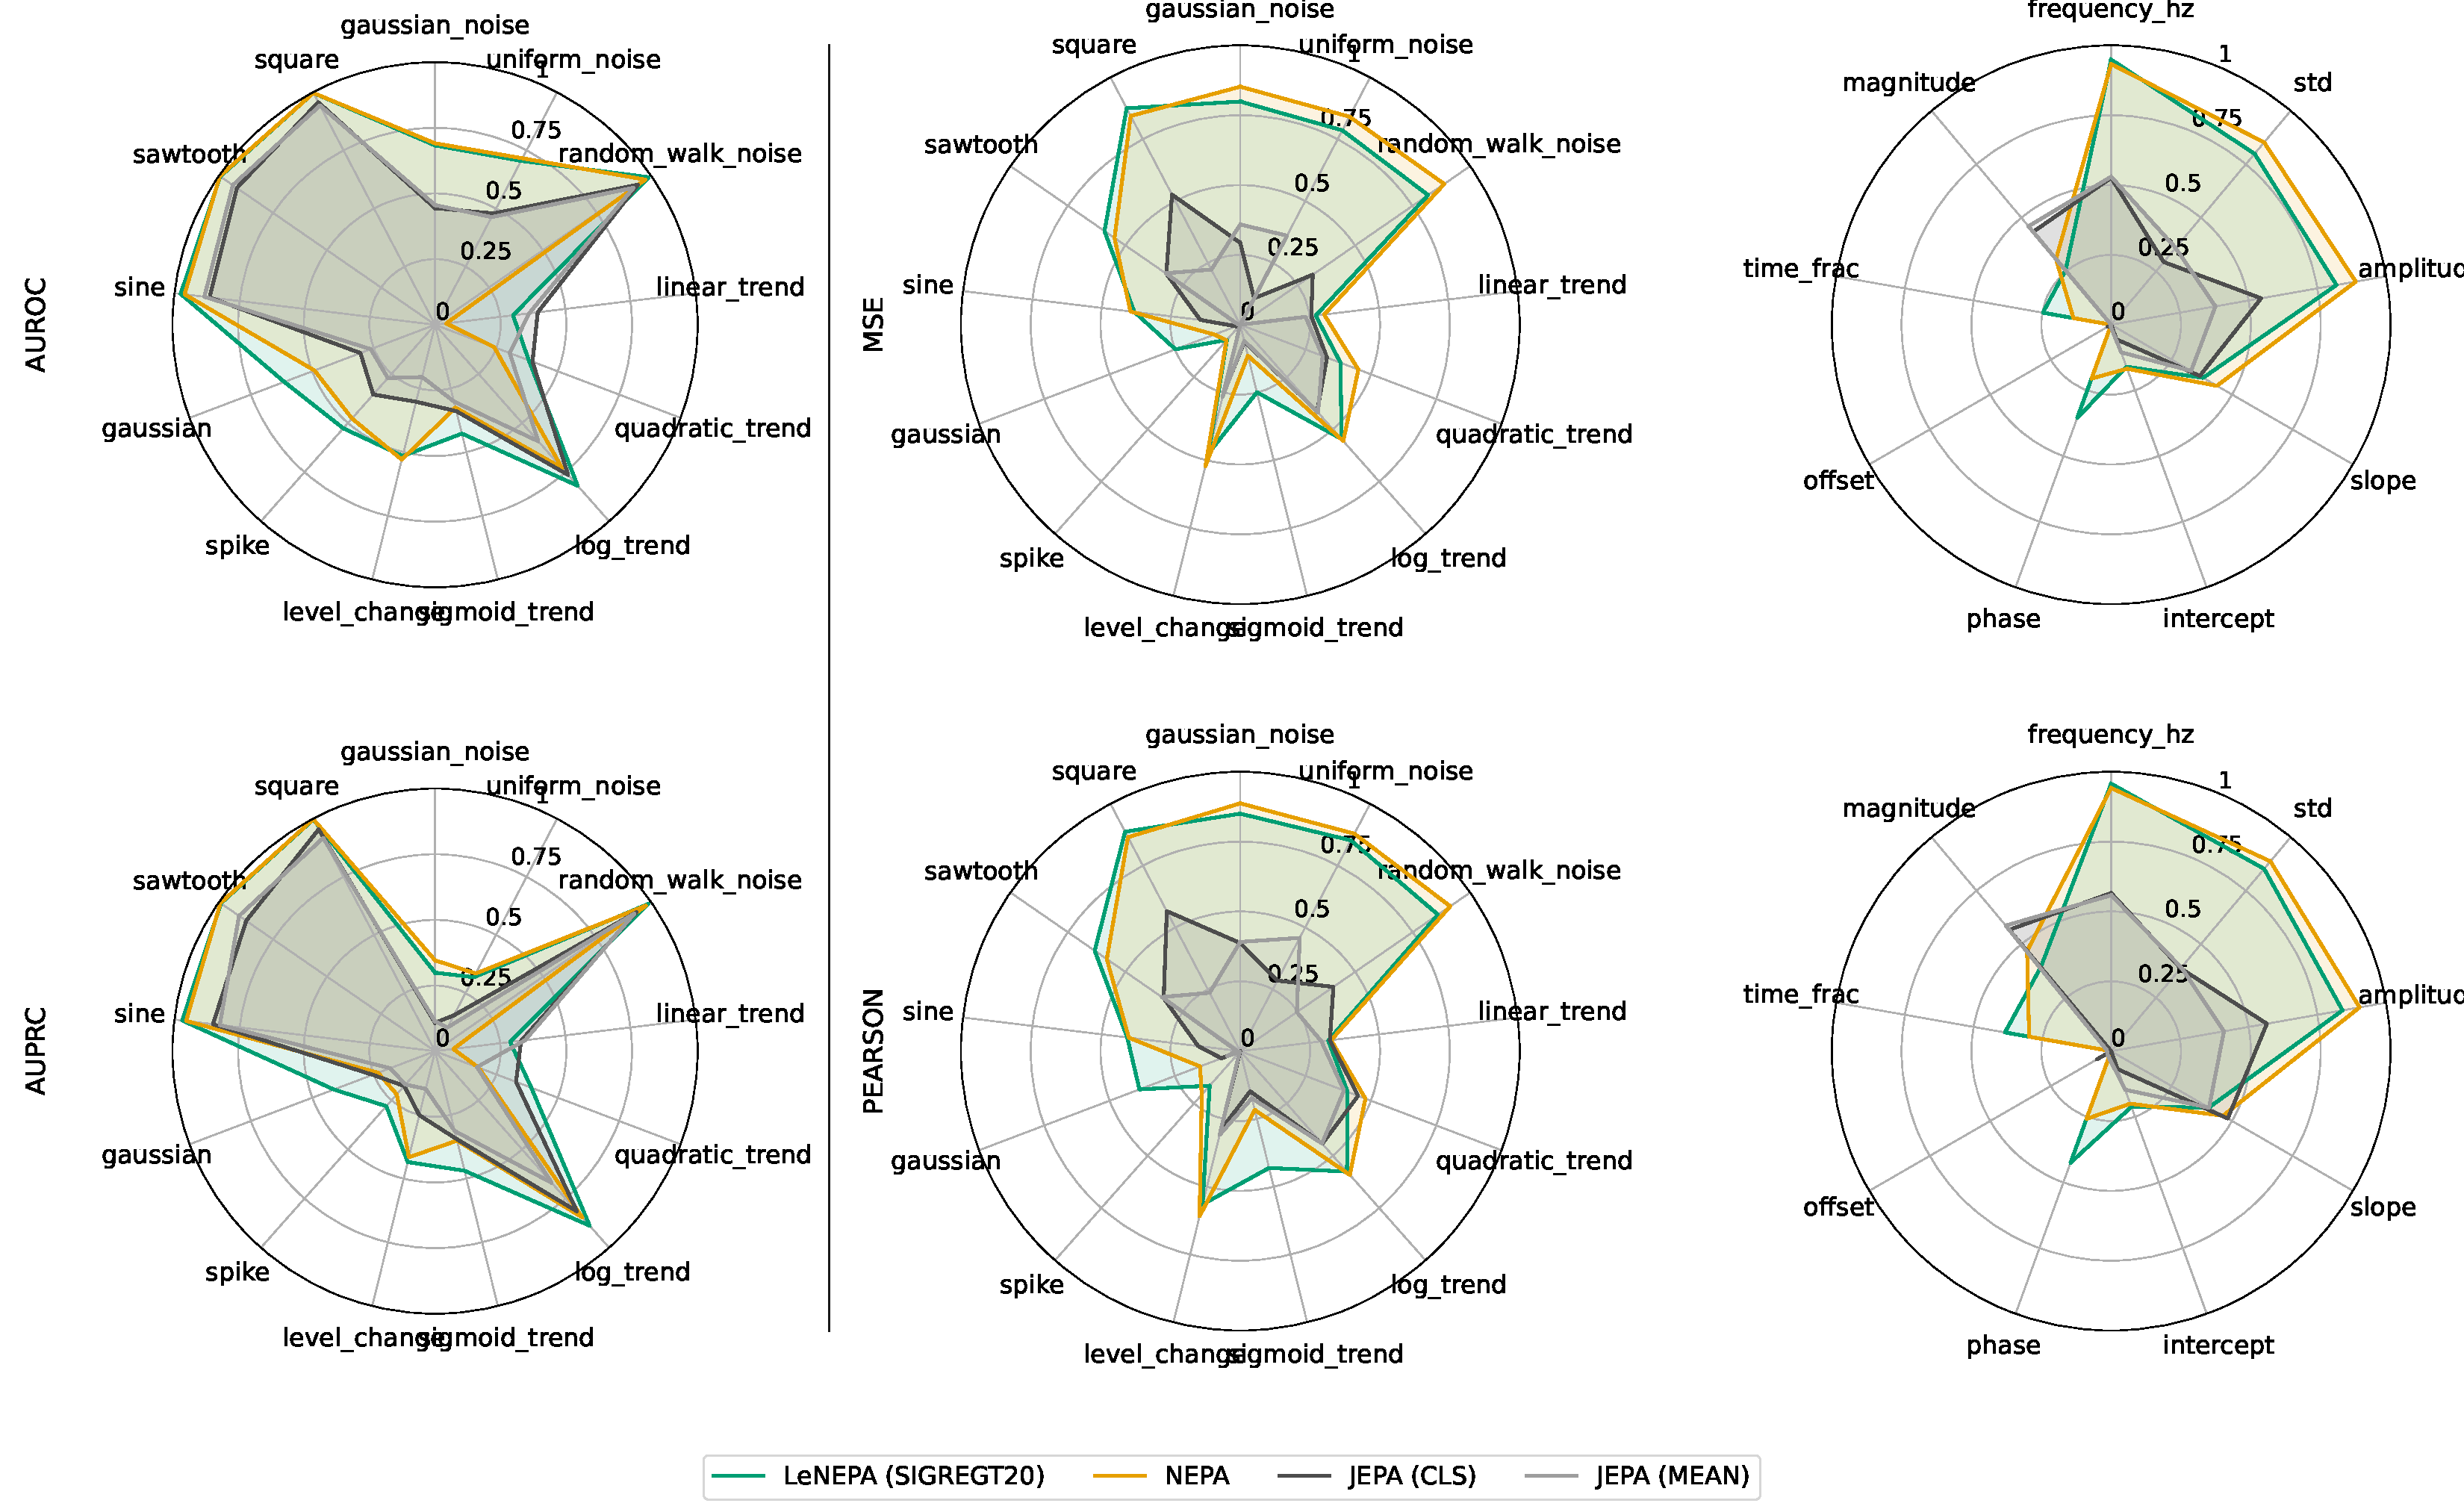
\includegraphics[width=\textwidth,height=0.40\textheight,keepaspectratio]{figures/aionoscope_balanced_basic_components_combined_radar_grid.pdf}
  \caption{Balanced sampler (uniform component weights).}
  \label{fig:aionoscope_balanced_basic_components_combined_radar_grid}
\end{subfigure}

\vspace{0.75em}

\begin{subfigure}{\textwidth}
  \centering
  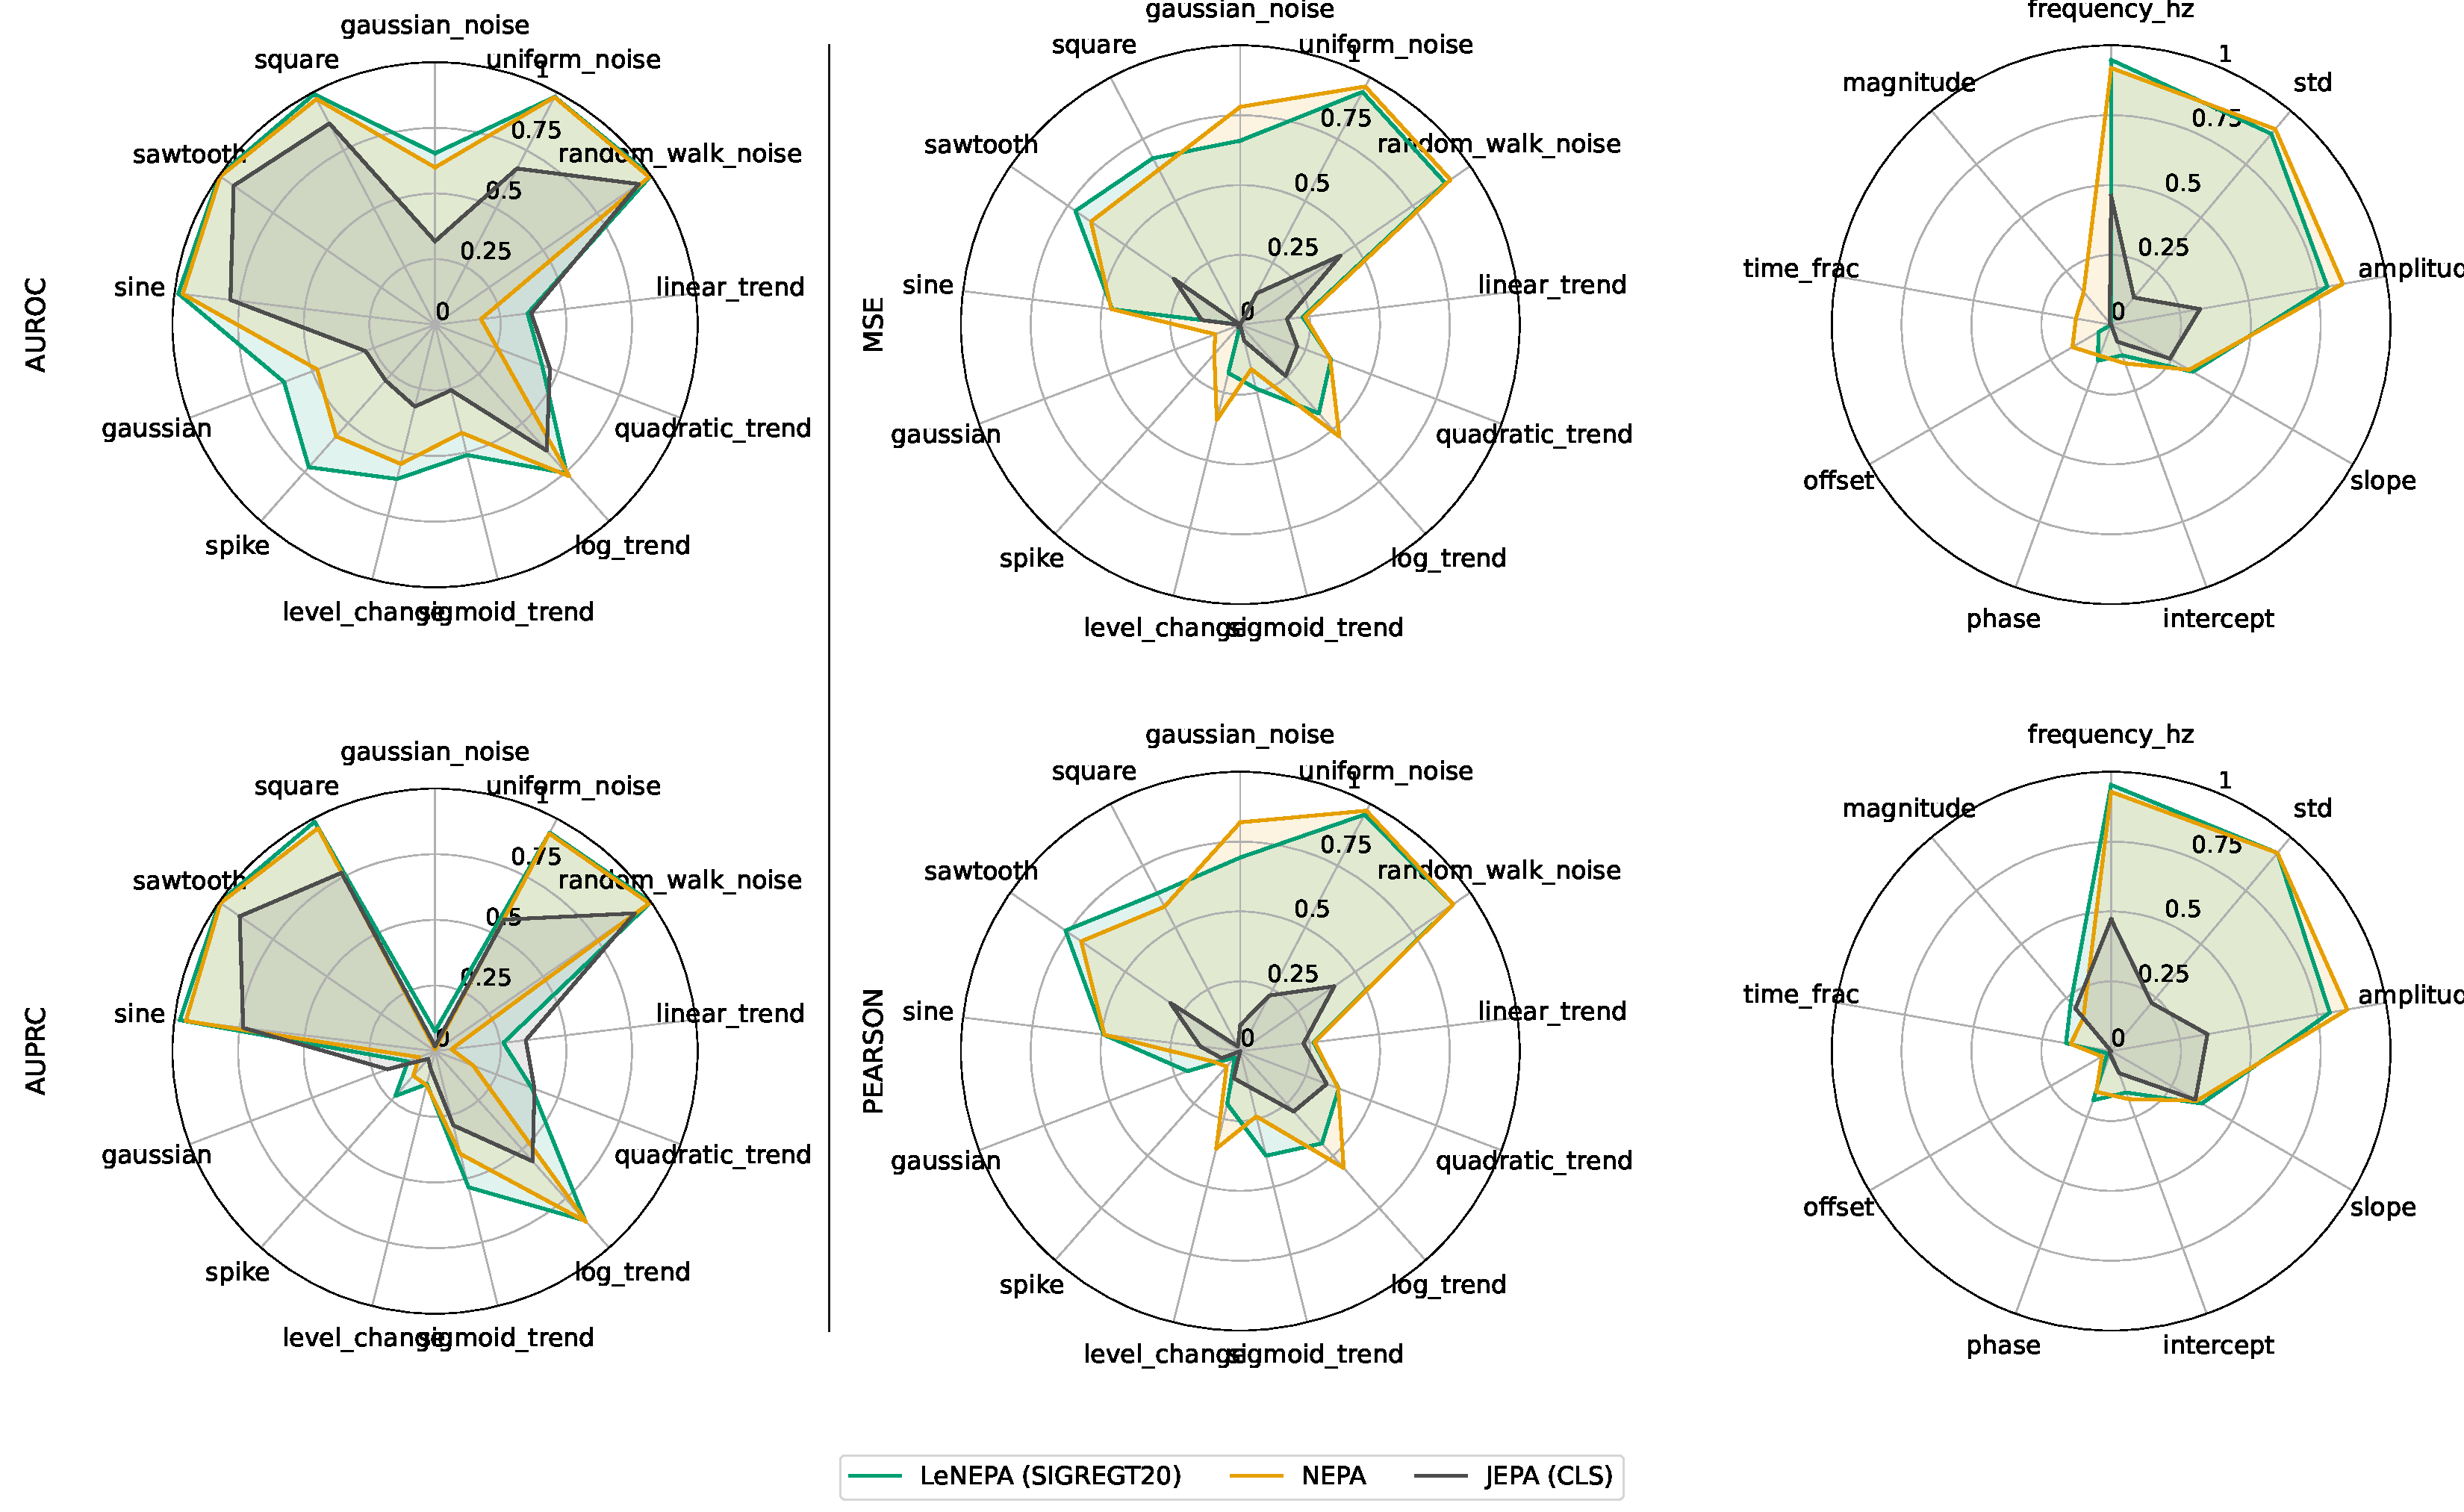
\includegraphics[width=\textwidth,height=0.40\textheight,keepaspectratio]{figures/aionoscope_combined_radar_grid.pdf}
  \caption{Imbalanced sampler with rare components.}
  \label{fig:aionoscope_combined_radar_grid}
\end{subfigure}

\caption{Aionoscope \emph{basic-components} signatures on (a) balanced and (b) imbalanced samplers. Panel (a) includes four objectives (LeNEPA T20, NEPA, JEPA CLS, JEPA MEAN); panel (b) includes LeNEPA T20, NEPA, and JEPA CLS. Left column: per-signal categorical improvements in best-layer AUROC (top) and AUPRC (bottom). Middle and right columns: dense improvements for MSE (top row) and Pearson (bottom row), aggregated by \texttt{target\_signal} families (middle) and by \texttt{target\_metric} types with $>1$ targets (right). For each signal/target we compute a step-$0$ normalized improvement between step $0$ and step $20{,}000$ using the best layer (layers $0$--$8$, selected independently at each step) and clamp scores to $[0,1]$. Dense panels report the median across targets within each group. Higher scores indicate larger relative improvements.}
\end{figure*}

\subsection{Experiment Matrix}
\label{sec:appendix_experiments_matrix}

Across two datasets (Aionoscope \emph{basic-components} and PTB-XL), we compare three families of self-supervised pretraining objectives:
\begin{itemize}
  \item \textbf{JEPA:} an augmentation-based JEPA baseline, evaluated with both CLS-token and mean-pooling readouts.
  \item \textbf{NEPA:} a next-embedding prediction baseline stabilized with stop-gradient (mean pooling).
  \item \textbf{LeNEPA:} our SIGReg-stabilized NEPA variant (mean pooling; no stop-gradient). We report two representative settings: (i) \texttt{T20 L0-8}, which uses temporal SIGReg with $\lambda_{\text{T}}=20$ applied to layers 0~(embedding) and 8~(last transformer layer); and (ii) \texttt{BRI20 L0-8}, which combines batch-wise, representation-level, and innovation SIGReg with $\lambda_{\text{B}}=\lambda_{\text{R}}=\lambda_{\text{I}}=20$ applied to layers 0~(embedding) and 8~(last transformer layer).
\end{itemize}
Appendix~\ref{sec:appendix_sigreg} defines the exact SIGReg placements and hyperparameters for these LeNEPA variants.
For NEPA/LeNEPA we additionally ablate the effect of the projector head by running each configuration with and without projection (controlled by \texttt{use\_projector}), yielding $8$ runs per dataset and $16$ runs total.

\subsection{Summary Plots}
\label{sec:appendix_experiments_summary}

To disentangle gains due to pretraining from the inherent behavior of the randomly initialized tokenizer+backbone (and dataset-specific baseline effects), we primarily report \emph{improvements over step $0$} rather than absolute last-step values.
Figure~\ref{fig:summary_last_step_delta_from_step0_bars} summarizes the best-layer delta between step $20{,}000$ and step $0$, selecting the best layer separately for each metric and step (over layers $0$--$8$). For MSE/MAE, negative values indicate improvement. Absolute last-step values are shown in Figure~\ref{fig:summary_last_step_bars}.

\begin{figure*}[t]
\centering
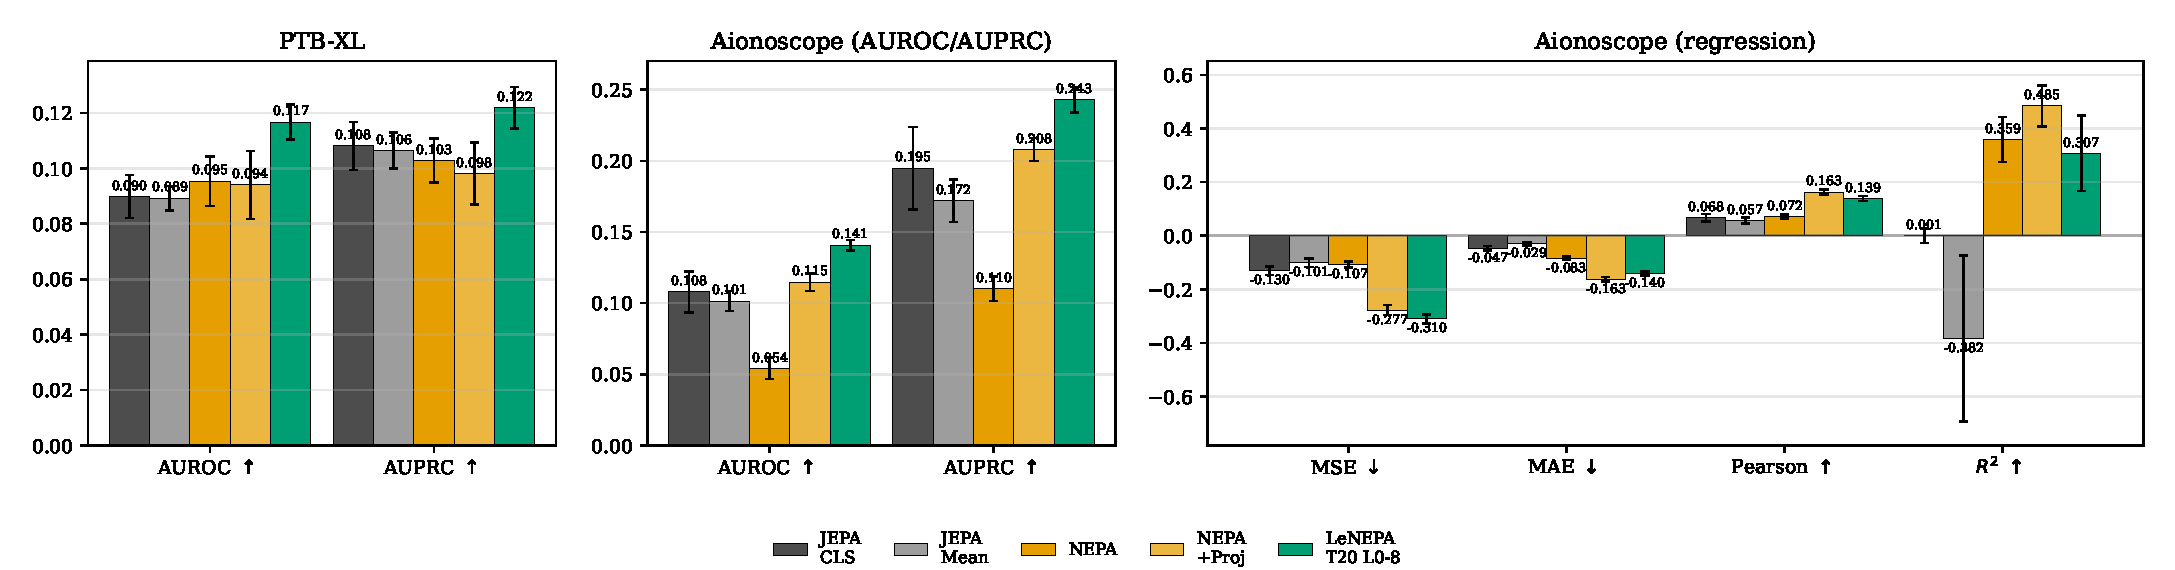
\includegraphics[width=\textwidth]{figures/summary_last_step_delta_from_step0_bars.pdf}
\caption{Last-step (step $20{,}000$) best-layer frozen-backbone probe deltas relative to step $0$ (untrained initialization) on PTB-XL and Aionoscope. For each method and metric, the reported value is the best score over probed layers $0$--$8$, selected separately at step $0$ and at the last step.}
\label{fig:summary_last_step_delta_from_step0_bars}
\end{figure*}

\begin{figure*}[t]
\centering
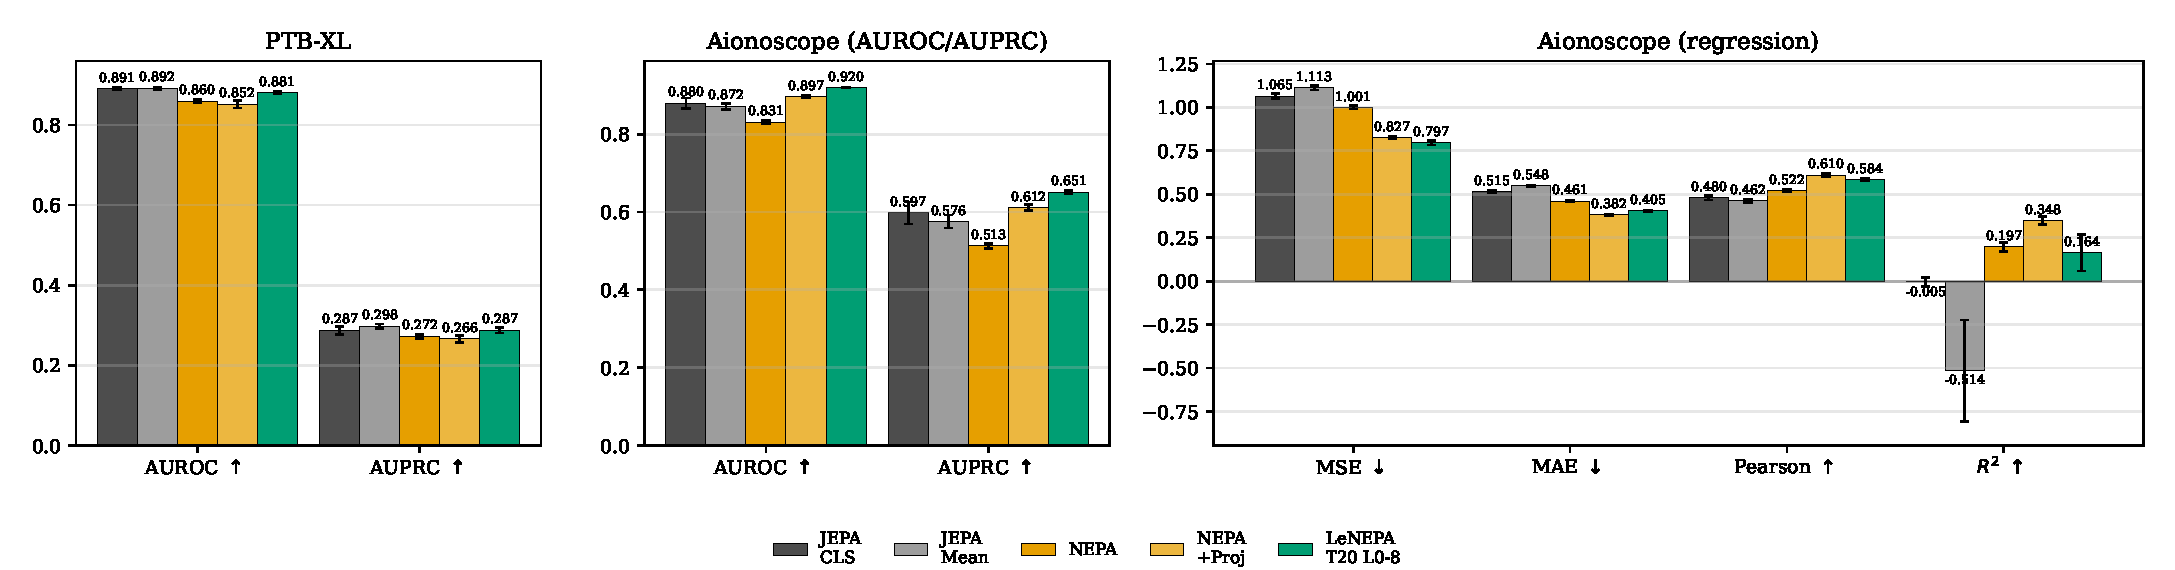
\includegraphics[width=\textwidth]{figures/summary_last_step_bars.pdf}
\caption{Absolute last-step (step $20{,}000$) best-layer frozen-backbone probe performance on PTB-XL and Aionoscope. Bars show macro AUROC/AUPRC for both datasets and MSE/MAE/Pearson/$R^2$ for Aionoscope. For each method and metric, the reported value is the best score over probed layers $0$--$8$.}
\label{fig:summary_last_step_bars}
\end{figure*}

\subsection{Projector Ablation}
\label{sec:appendix_experiments_projector}

We ablate the LeNEPA/NEPA projector $h_{\psi}$ (Appendix~\ref{sec:appendix_projector}), inspired by Guillotine Regularization~\citep{bordes2022guillotine}, by comparing variants that compute the predictive loss (and, when applicable, SIGReg) in a projected space (\texttt{use\_projector=true}) versus directly in backbone token space (\texttt{use\_projector=false}).
Table~\ref{tab:projector_ablation_last_step} reports last-step best-layer probe metrics for no-projector ($-$) versus projector ($+$) variants.

\begin{table}[t]
\centering
\scriptsize
\caption{Projector ablation (NEPA / LeNEPA): best-layer value at the last \emph{common} offline-probe eval step across seeds and projector toggles, aggregated across seeds as $\mathrm{median}(\mathrm{std})$ (ddof=1; std shown in $10^{-3}$ units). Each cell reports $-\mathrm{Proj} / +\mathrm{Proj}$; within each pair, the better value by median is bold (higher is better for AUROC / AUPRC / Pearson / $R^2$; lower is better for MSE / MAE).}
\label{tab:projector_ablation_last_step}

\setlength{\tabcolsep}{3pt}
\renewcommand{\arraystretch}{1.15}
\resizebox{\linewidth}{!}{%
\begin{tabular}{lllrrrrrr}
\toprule
& & & \multicolumn{2}{c}{Classification} & \multicolumn{4}{c}{Dense regression} \\
\cmidrule(lr){4-5}\cmidrule(lr){6-9}
dataset & model & config & AUROC & AUPRC & MSE & MAE & Pearson & $R^2$ \\
\midrule
\multirow{3}{*}{PTB-XL} & NEPA &  & \textbf{0.860(3)} / 0.852(9) & \textbf{0.272(5)} / 0.266(8) & \multicolumn{4}{c}{\textemdash} \\
& LeNEPA & T20 L0-8 & 0.864(4) / \textbf{0.881(3)} & 0.259(4) / \textbf{0.287(6)} & \multicolumn{4}{c}{\textemdash} \\
& LeNEPA & BRI20 L0-8 & 0.832(7) / \textbf{0.863(4)} & 0.245(5) / \textbf{0.278(6)} & \multicolumn{4}{c}{\textemdash} \\
\midrule
\multirow{3}{*}{Aionoscope} & NEPA &  & 0.831(4) / \textbf{0.897(2)} & 0.513(6) / \textbf{0.612(7)} & 1.001(9) / \textbf{0.827(8)} & 0.461(3) / \textbf{0.382(3)} & 0.522(4) / \textbf{0.610(7)} & 0.197(24) / \textbf{0.348(23)} \\
& LeNEPA & T20 L0-8 & 0.848(3) / \textbf{0.920(1)} & 0.588(11) / \textbf{0.651(4)} & 0.886(32) / \textbf{0.797(12)} & 0.449(18) / \textbf{0.405(4)} & 0.519(17) / \textbf{0.584(6)} & -0.214(138) / \textbf{0.164(105)} \\
& LeNEPA & BRI20 L0-8 & 0.868(6) / \textbf{0.902(1)} & 0.567(9) / \textbf{0.608(3)} & 0.975(10) / \textbf{0.834(10)} & 0.502(4) / \textbf{0.396(4)} & 0.488(7) / \textbf{0.590(6)} & -0.767(337) / \textbf{-0.437(228)} \\
\bottomrule
\end{tabular}
} % resizebox
\end{table}


Across the $24$ metric comparisons in Table~\ref{tab:projector_ablation_last_step} (two PTB-XL metrics and six Aionoscope metrics for each of three configurations), projector-enabled variants are better in $22/24$ cases.
The only exception is NEPA on PTB-XL classification, where the no-projector variant is slightly better.
Therefore, in the remainder of this work we use LeNEPA \emph{only} with the projector enabled, and report both NEPA and NEPA~+Proj for clarity.

\subsection{SIGReg Component Ablations}
\label{sec:appendix_experiments_sigreg_component_ablations}

To isolate the effect of each SIGReg placement (Appendix~\ref{sec:appendix_sigreg}), we run LeNEPA with exactly one SIGReg component enabled at scale $20$ (projector enabled; \texttt{pred\_depth=0}; seed $0$) while keeping the predictive loss $\mathcal{L}_{\text{pred}}$ unchanged.
Concretely, using the notation from Appendix~\ref{sec:appendix_sigreg}, we denote by $u^{(\ell)}\in\mathbb{R}^{B\times T\times d}$ the projected patch-token embeddings at layer $\ell$ (after the optional projector $h_{\psi}$), and we set $\lambda_{\text{pred}}=1$ and enable exactly one of $\{\lambda_{\text{B}},\lambda_{\text{T}},\lambda_{\text{R}},\lambda_{\Delta},\lambda_{\text{BT}}\}$ at value $20$, with all other SIGReg scales set to $0$ in Eq.~\eqref{eq:sigreg_total}.
We use $\mathcal{L}_{\text{B}}=\mathcal{L}_{\text{T}}=\mathcal{L}_{\Delta}=\mathcal{L}_{\text{BT}}=\{0,8\}$ and $\mathcal{L}_{\text{R}}=\{8\}$, matching the layer choices in the main matrix.

\paragraph{Single-component variants.}
\begin{itemize}
  \item \textbf{\texttt{B20} (batch-wise SIGReg).} We regularize the distribution across the batch at each time index (Eq.~\eqref{eq:sigreg_batch}), encouraging non-collapsed embeddings across samples while preserving the temporal structure within each sample.
  \item \textbf{\texttt{T20} (temporal SIGReg).} We regularize the distribution across time for each sample (Eq.~\eqref{eq:sigreg_time}), explicitly discouraging per-sample temporal collapse where token embeddings become nearly constant over the time axis.
  \item \textbf{\texttt{R20} (representation-level SIGReg).} We apply SIGReg to pooled per-layer sequence representations $r^{(\ell)}$ (Eq.~\eqref{eq:sigreg_rep}), using the same readout as for linear probing. In our setup this is mean pooling over patch tokens, $r^{(\ell)}_b=\frac{1}{T}\sum_{t=1}^{T}u^{(\ell)}_{b,t}$. This placement is the closest to the original LeJEPA use of SIGReg~\citep{balestriero2025lejepa}, which regularizes a single representation vector per sample/view rather than token sequences.
  \item \textbf{\texttt{I20} (innovation SIGReg).} We apply SIGReg to innovations $\Delta u^{(\ell)}_{b,t}=u^{(\ell)}_{b,t+1}-u^{(\ell)}_{b,t}$ (Eq.~\eqref{eq:sigreg_innov_def}--\eqref{eq:sigreg_innov}), regularizing dynamics (temporal differences) rather than absolute token values.
  \item \textbf{\texttt{BT20} (batch-time SIGReg).} We flatten batch and time and apply SIGReg to the joint set of tokens per layer (Eq.~\eqref{eq:sigreg_batch_time}). Relative to \texttt{B20} and \texttt{T20}, this is a more relaxed axis-agnostic constraint: it enforces global non-collapse across all token instances while avoiding explicit per-time-index (\texttt{B20}) or per-sample temporal (\texttt{T20}) regularization, serving as a check that our conclusions are not driven by over-regularizing along a specific axis.
\end{itemize}

\paragraph{Layer placement relative to $\mathcal{L}_{\text{pred}}$.}
In our main LeNEPA setup, the prediction loss $\mathcal{L}_{\text{pred}}$ (Eq.~\eqref{eq:lenepa_pred}) aligns predicted tokens from the top backbone layer ($\ell=8$) with next-step targets taken from the tokenizer embedding layer ($\ell=0$).
We observed that applying SIGReg to both sides of this regression (i.e., regularizing layers $\{0,8\}$) yields more transferable frozen-backbone representations in most cases than applying SIGReg only on the prediction side (layer $8$).
In contrast, applying SIGReg only to the embedding targets (layer $0$) yields substantially weaker transfer.
More generally, applying SIGReg to layers that do not participate in $\mathcal{L}_{\text{pred}}$ (e.g., intermediate layers when targets are taken from $\ell=0$) leads to collapse or severely degraded transfer.
We omit plots for these additional ablations due to space constraints.
We hypothesize that SIGReg is most effective when it directly counterbalances the prediction objective in the same embedding space as $\mathcal{L}_{\text{pred}}$, rather than regularizing features that are not directly tied to the regression targets.

Finally, we compare these single-component variants to the multi-term reference configuration \texttt{BRI20} used in the main matrix ($\lambda_{\text{B}}=\lambda_{\text{R}}=\lambda_{\Delta}=20$ with the layer sets above).
Figure~\ref{fig:sigreg_component_ablations_dynamics} reports best-layer transfer dynamics (over layers $0$--$8$).
The top row shows AUROC/AUPRC for PTB-XL and Aionoscope, while the bottom row shows Aionoscope dense-target metrics (MSE/MAE/Pearson/$R^2$).
In our setup, temporal SIGReg is the only single-component placement that consistently yields sustained improvements in frozen-backbone transfer performance across both datasets.

\begin{figure*}[t]
\centering
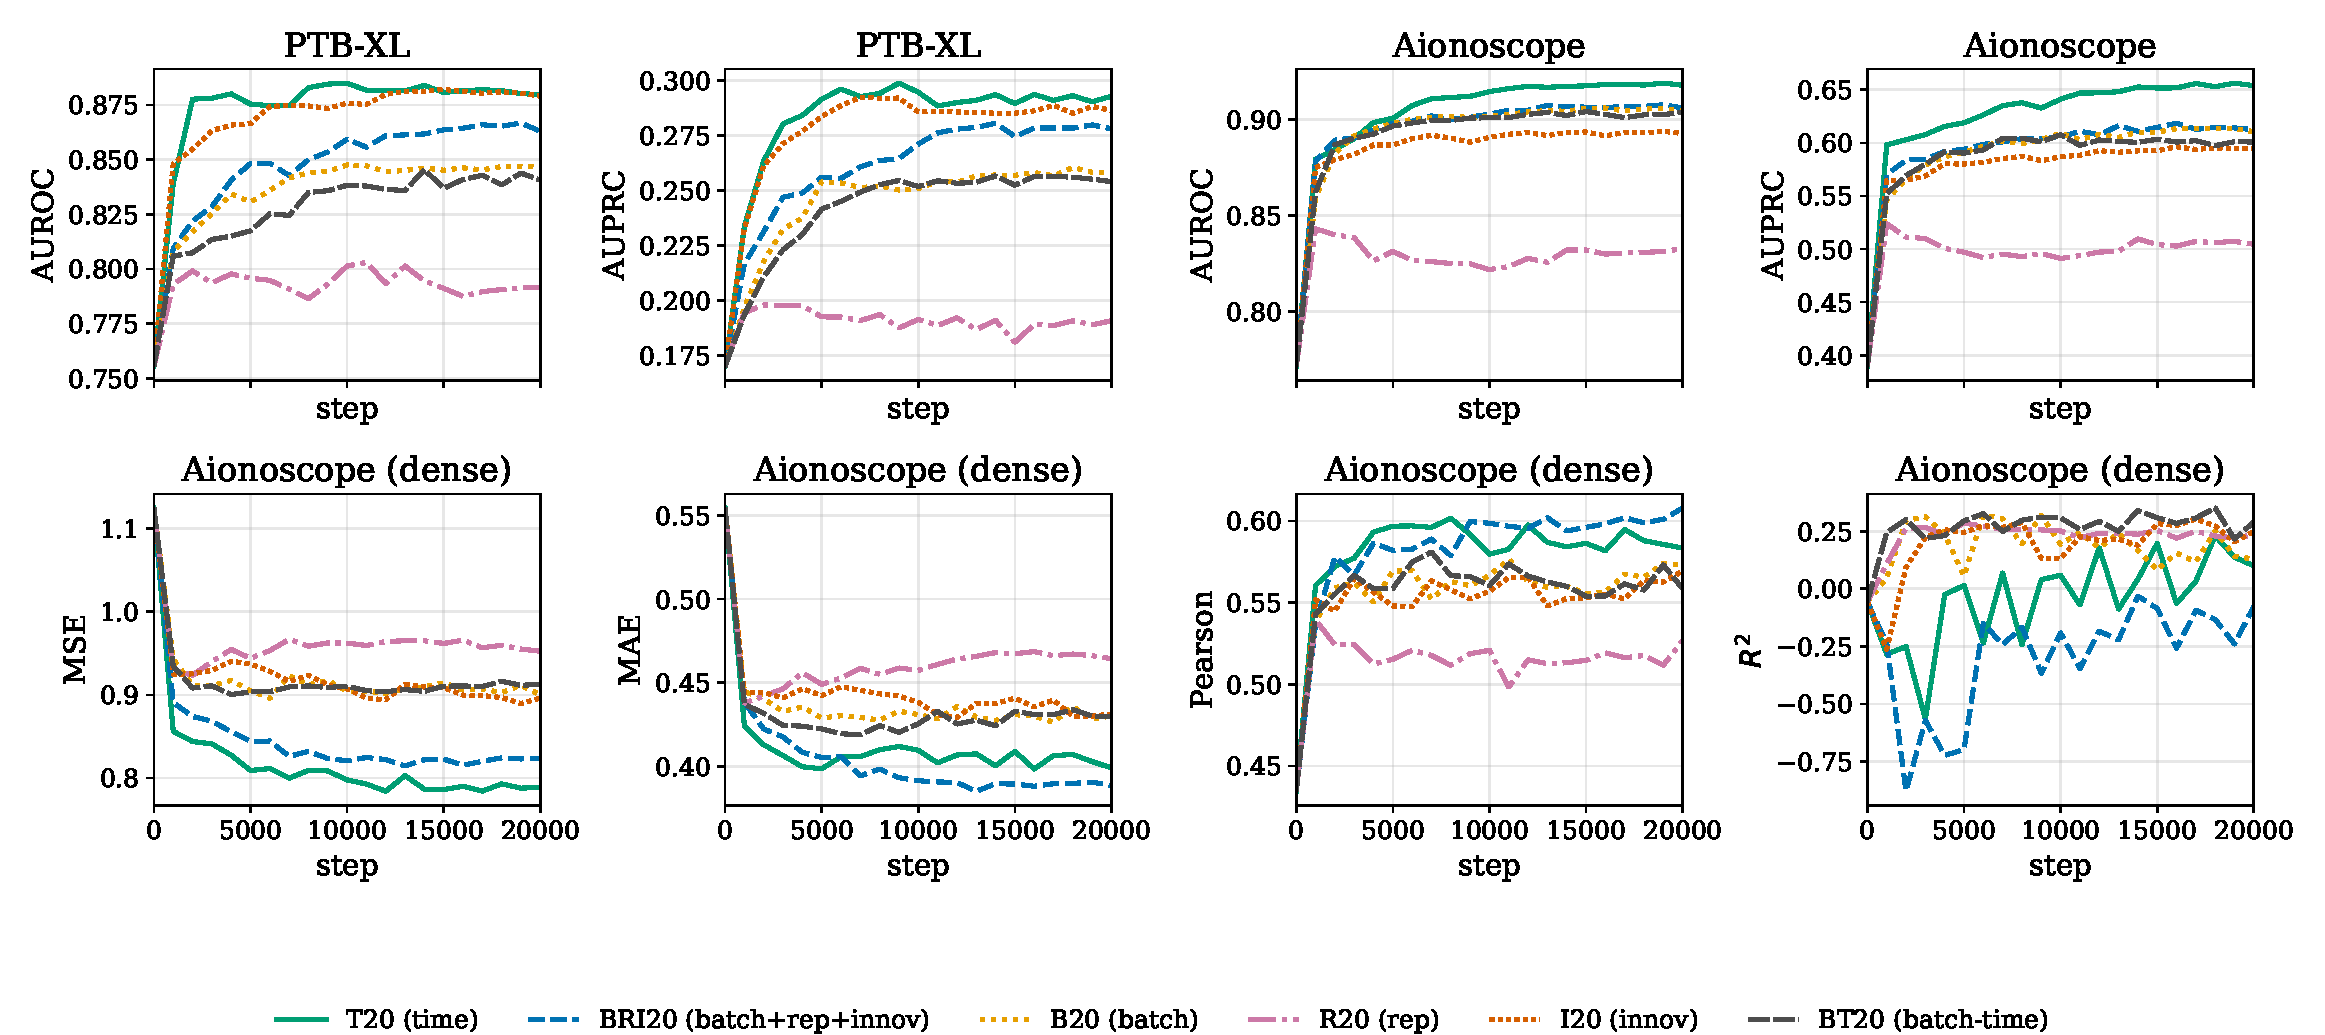
\includegraphics[width=\textwidth]{figures/sigreg_component_ablations_dynamics.pdf}
\caption{SIGReg component ablations (seed $0$ only; projector enabled): best-layer transfer dynamics for time-only (\texttt{T20}), batch-only (\texttt{B20}), representation-only (\texttt{R20}), innovation-only (\texttt{I20}), batch-time-only (\texttt{BT20}), and the multi-term reference configuration (\texttt{BRI20}). Top row: classification AUROC/AUPRC for PTB-XL and Aionoscope. Bottom row: Aionoscope dense-target metrics (MSE/MAE/Pearson/$R^2$), where lower is better for MSE/MAE. Best layer is selected independently at each step (over layers $0$--$8$).}
\label{fig:sigreg_component_ablations_dynamics}
\end{figure*}

\subsection{Aionoscope Dense Target Training Dynamics}
\label{sec:appendix_experiments_aionoscope_dense_dynamics}

Figure~\ref{fig:aionoscope_dynamics_best_layer_dense} reports training dynamics for dense regression targets on the Aionoscope \emph{basic-components} benchmark.
For each metric and each offline-probe evaluation step, we plot the best-layer value over probed layers $0$--$8$.

\begin{figure*}[t]
\centering
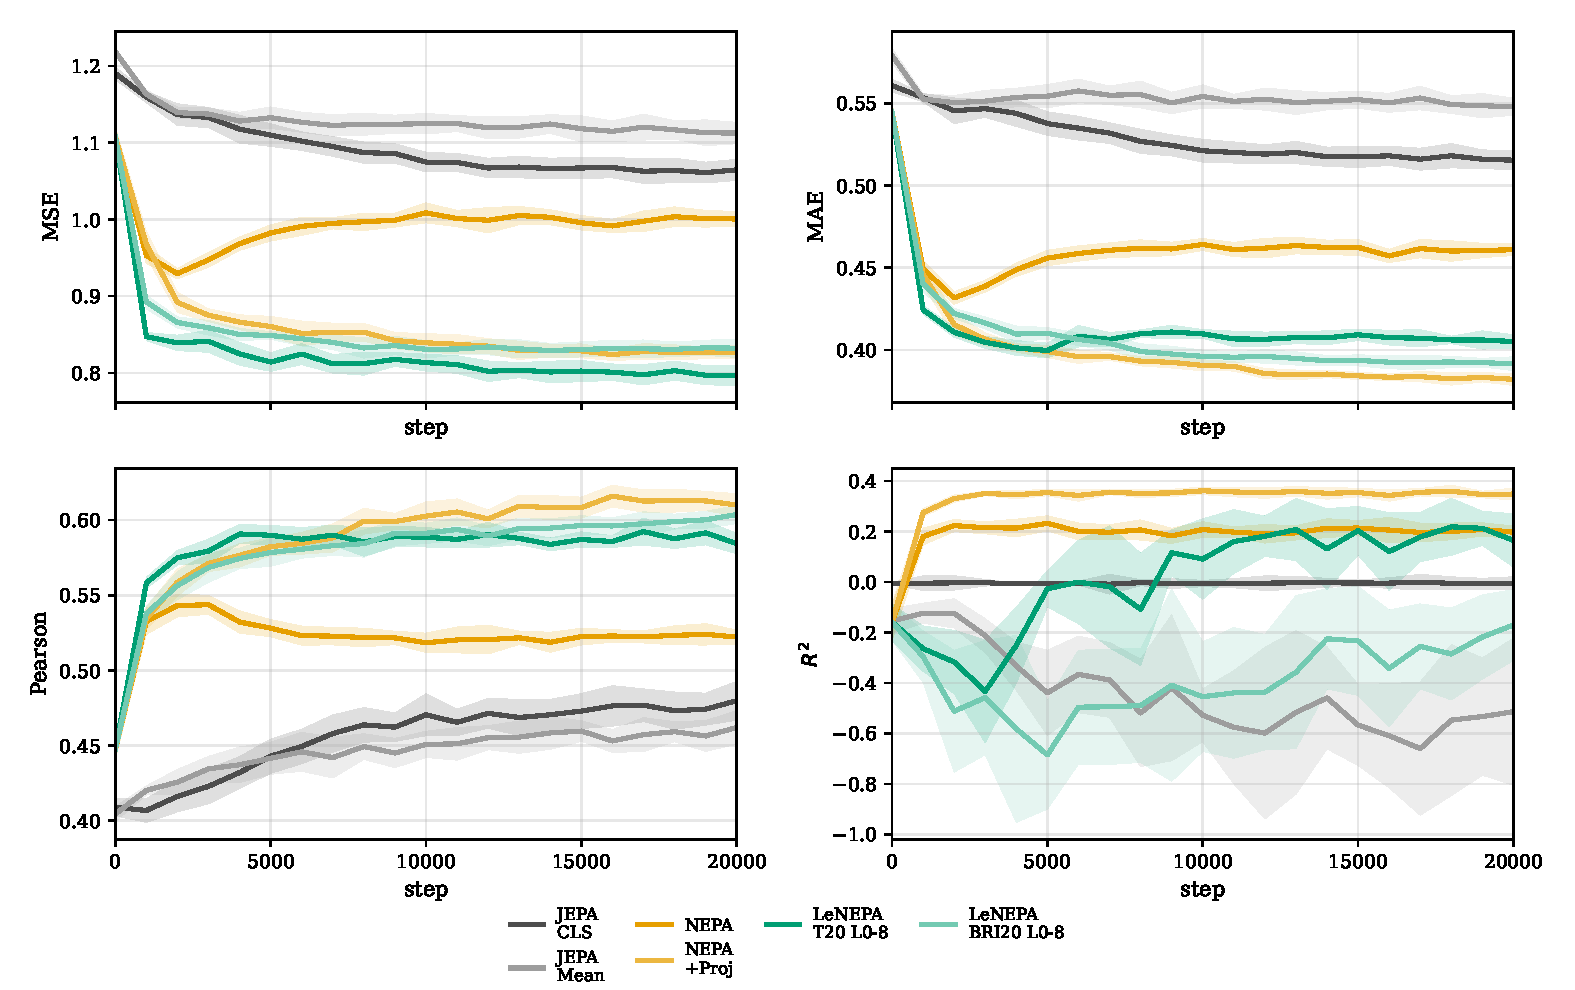
\includegraphics[width=\textwidth]{figures/aionoscope_dynamics_best_layer_dense.pdf}
\caption{Aionoscope \emph{basic-components} dense-target dynamics: best-layer over layers $0$--$8$ frozen-backbone probe performance over training steps for MSE/MAE/Pearson/$R^2$.}
\label{fig:aionoscope_dynamics_best_layer_dense}
\end{figure*}

\subsection{JEPA Masking Fragility}
\label{sec:appendix_experiments_jepa_masking_fragility}

JEPA relies on a masking-based view construction controlled by a keep-ratio range, $\rho \sim \mathrm{Uniform}(\rho_{\min}, \rho_{\max})$, which determines the fraction of tokens retained in the context view.
To illustrate the sensitivity of augmentation-driven SSL in time series, we rerun the PTB-XL JEPA (CLS) configuration with two alternative keep-ratio ranges:
(i) a more aggressive masking regime $(\rho_{\min},\rho_{\max})=(0.05,0.10)$ and
(ii) a lighter masking regime $(\rho_{\min},\rho_{\max})=(0.30,0.40)$, compared to the baseline $(0.15,0.25)$ used throughout the paper.
All other hyperparameters, including the $20{,}000$-step fixed-horizon protocol and the layer-wise offline probing setup, are kept identical. The resulting best-layer AUROC/AUPRC training dynamics are shown in Figure~\ref{fig:ptbxl_jepa_masking_fragility_dynamics}.
As we can see, changing the augmentation parameters by just $2$--$3\times$ leads to a significant degradation in the representation quality.

\begin{figure*}[t]
\centering
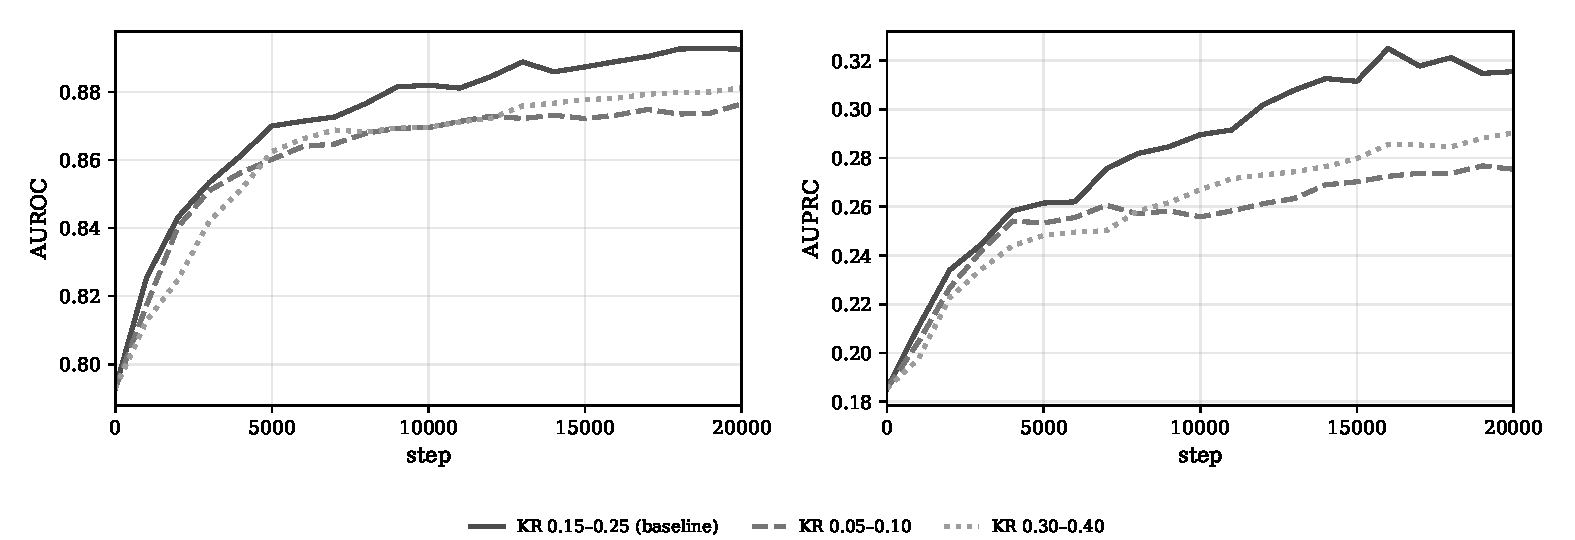
\includegraphics[width=\textwidth]{figures/ptbxl_jepa_masking_fragility_dynamics.pdf}
\caption{PTB-XL JEPA masking fragility (seed $0$ only): best-layer AUROC/AUPRC dynamics under different keep-ratio ranges (selected over layers $0$--$8$ at each step).}
\label{fig:ptbxl_jepa_masking_fragility_dynamics}
\end{figure*}


\end{document}
